\documentclass[11pt,a4paper]{article}

% Clean Supplementary Information layout based on the standard article class
% recommended by Nature Energy for TeX/LaTeX manuscripts.
\usepackage{graphicx}
\usepackage{amsmath,amssymb,amsfonts}
\usepackage{xcolor}
\usepackage{textcomp}
\usepackage{booktabs}
\usepackage{array}
\usepackage{tabularx}
\usepackage{longtable}
\usepackage{placeins}
\usepackage{xurl}
\usepackage[numbers,sort&compress]{natbib}
\usepackage[font=small,labelfont=bf]{caption}
\usepackage[hidelinks]{hyperref}
\usepackage[a4paper,left=24mm,right=24mm,top=22mm,bottom=22mm,footskip=10mm]{geometry}

\raggedbottom
\setlength{\emergencystretch}{2em}
\setlength{\parindent}{0pt}
\setlength{\parskip}{0.5em plus 0.08em minus 0.05em}
\setlength{\bibsep}{0.35em}
\renewcommand{\arraystretch}{1.15}
\makeatletter
\setlength{\@fptop}{0pt}
\setlength{\@fpsep}{12pt}
\setlength{\@fpbot}{0pt plus 1fil}
\renewcommand*{\l@section}{\@dottedtocline{1}{0em}{3em}}
\makeatother
\pagestyle{plain}
\renewcommand{\thesection}{S\arabic{section}}
\renewcommand{\thesubsection}{\thesection.\arabic{subsection}}
\renewcommand{\thefigure}{S\arabic{figure}}
\renewcommand{\thetable}{S\arabic{table}}
\renewcommand{\theequation}{S\arabic{equation}}

\newcommand{\Htwo}{H$_2$}
\newcommand{\cnykg}{CNY\,kg$^{-1}$}
\newcommand{\cnykwh}{CNY\,kWh$^{-1}$}
\newcommand{\lowhurdle}{approximately 1.45\%}
\newcommand{\dataset}{project-record inventory}

\begin{document}

\title{Supplementary Information for\\
Curtailment traps early green hydrogen assets beyond the reach of learning}
\author{Jinwei Liang$^{1,2,\dagger}$, Zhiling Guo$^{3}$ and Haoran Zhang$^{1,2,*,\dagger}$\\[0.65em]
\small $^{1}$School of Urban Planning and Design, Peking University, Shenzhen, China\\
\small $^{2}$Guangdong Provincial Key Laboratory of Risk Perception and Sustainable Governance\\
\small in Energy Transition, Shenzhen, China\\
\small $^{3}$Department of Building Environment and Energy Engineering,\\
\small The Hong Kong Polytechnic University, Hong Kong, China\\[0.45em]
\small $^{*}$Corresponding author: \href{mailto:h.zhang@pku.edu.cn}{h.zhang@pku.edu.cn}\\
\small $^{\dagger}$These authors contributed equally to this work.}
\date{}

\maketitle

\begin{abstract}
This Supplementary Information provides the complete data lineage, hourly resource reconstruction, electrolyser dispatch, capacity search, nominal equity-cash-flow model, vintage-specific learning treatment, scenario definitions, robustness tests, interpretation audit and numerical quality controls supporting the main manuscript. Record counts describe conditional exposure within the covered inventory rather than national investment forecasts. All scenario grids are deterministic unless explicitly stated; scenario frequencies are not probabilities.
\end{abstract}

\noindent\textbf{Keywords:} green hydrogen; low-opportunity-cost electricity; project finance; learning curves; vintage capital; capacity flexibility
\vspace{1em}

\section*{Guide to this Supplementary Information}

This file is organised as Supplementary Methods S1--S10, Supplementary Notes 1--12, Supplementary Tables S1--S12 and Supplementary Figures S1--S4. The primary analysis specification is denoted \textbf{M129}: 128 nested resource-capture candidates plus the exact 1-MW engineering boundary for each of 10,214 project records. Broad deterministic grids using 16 capacity candidates are denoted \textbf{G16} and are used only for directional sensitivity ranges. Results from M129 and G16 are never pooled and always retain their own denominator. Supplementary Note 12 and Supplementary Table S12 provide a reviewer-facing audit that distinguishes questions answered by the present evidence from boundaries that require new observations or a larger system model.

The primary numerical source is \path{source_data/headline_results.json}. Supporting machine-readable files accompany this document in the \texttt{source\_data} directory. Values in the prose are rounded to precision commensurate with model uncertainty; the source files retain full numerical precision for reproducibility.

\begingroup
\footnotesize
\setlength{\parskip}{0pt}
\tableofcontents
\endgroup

\clearpage

\section{Data sources, analysis unit and sample boundary}\label{sec:data}

\subsection{Project-record inventory}

The analysis unit is an \texttt{ObjectId} record from the June 2024 releases of the Global Wind Power Tracker and Global Solar Power Tracker maintained by Global Energy Monitor (GEM)\cite{gem2024}. The inventory contains 4,149 operating onshore-wind records and 6,065 operating utility-scale photovoltaic records, for 10,214 records and approximately 629\,GW in total. An \texttt{ObjectId} is unique within the inventory, but separate construction phases of one named facility can appear as multiple records. We therefore describe the units as \emph{project records}, not as 10,214 distinct physical plants. Exact parent-name grouping and coordinate duplication are used as diagnostics, not as an unvalidated deduplication rule.

Relative to official June 2024 capacities, the inventory represents approximately 63\% of all grid-connected wind and 83\% of centralized photovoltaics, or 72\% of the combined all-wind-plus-centralized-photovoltaic benchmark\cite{nea2024capacity}. Against the broader denominator that also includes distributed photovoltaics outside the inventory, the ratio is 53\%. Neither ratio is a sampling weight: distributed photovoltaics, later additions and assets absent from the tracker remain under-represented. Every absolute resource, capacity, capital and hydrogen quantity in this study is therefore conditional on this inventory. It is not a national census and must not be quoted as a forecast of total Chinese green hydrogen potential.

\subsection{Resource branches}

The main analysis uses only electricity reconstructed as system-constrained renewable output. A mutually exclusive full-output branch redirects all modelled wind and photovoltaic generation to electrolysis and charges the provincial feed-in price as an opportunity-cost proxy. The full-output branch is a physical and economic upper-bound experiment: it neither assumes that existing power-sale arrangements can be cancelled without friction nor adds to the constrained-output branch.

\subsection{Figure 1 map preparation}

Figure~1a separates the analytical main map from a boxed South China Sea locator inset. The main-map land layer is the intersection of coastline-derived OpenStreetMap polygons with OSM national administrative relations, and province lines are reconstructed from OSM admin-level-4 relations\cite{osmcoast}. Record coordinates and all main-map layers are transformed with the same China Albers equal-area projection (central meridian 105$^\circ$ E; standard parallels 25$^\circ$ and 47$^\circ$ N), eliminating cross-source registration within the analytical map. The South China Sea locator is a cleaned display derivative of the Ministry of Natural Resources standard-map product GS(2023)2767\cite{mnrmap2023}. It retains the source island and coastline geometry while suppressing small labels for legibility; it is not projected onto the analytical map and is not used for masking, record assignment, distance measurement or any numerical result. Both sources are used as cartographic context rather than legal boundary adjudication. The OSM queries, data timestamp, relation identifiers, standard-map product number, processing scripts, derived assets and SHA-256 hashes are packaged with the figure data; no analytical result depends on boundary placement.

\begin{table}[t]
\caption{Primary data sources, transformations and interpretation boundaries.}\label{tab:data}
\centering
\footnotesize
\begin{tabularx}{\textwidth}{>{\raggedright\arraybackslash}p{0.18\textwidth}>{\raggedright\arraybackslash}p{0.22\textwidth}>{\raggedright\arraybackslash}X>{\raggedright\arraybackslash}p{0.22\textwidth}}
\toprule
Input & Source or version & Transformation & Permitted interpretation \\
\midrule
Wind and solar inventory & GEM, June 2024 release\cite{gem2024} & Operating records selected; province and technology harmonised & Conditional inventory of project records, not a current national plant census \\
Reference hourly profiles & Laboratory-generated model-output files previously used by Li and Zhang, 2020, 8,784 h\cite{li2026} & Grid-delivered and constrained components summed only to recover pre-allocation full output & Research-group reference shape; neither component is treated as observed unit-level dispatch \\
Annual renewable utilisation & Provincial, technology-specific 2025 monitoring data\cite{renewable2025} & Converted to constrained-energy shares & Annual energy calibration; does not identify hourly constrained events \\
Meteorology & ERA5 hourly single levels, 2020--2025, 0.25$^\circ$\cite{hersbach2020,era5data} & Bilinear interpolation and generic wind/PV conversion & Weather-shape replay with utilisation rates held fixed \\
Installed-system CAPEX & World Bank installed-system range, converted to CNY\cite{worldbank2026} & Central and low/high deterministic cases & Complete alkaline-system boundary; IEA China quotations are contextual only\cite{iea2025} \\
Electrolyser operation & US DOE and World Bank assessments\cite{doe2024,worldbank2026} & Alkaline main case; PEM as a separate technology boundary & Technology-informed scenarios, not manufacturer guarantees \\
Return criteria & Official investment-management rules publicly disclosed by two state-controlled energy companies and ChinaBond yield observations\cite{changyuan2026,huadian2025,chinabond2026} & 20-trading-day mean for the five-year government bond anchor & Firm-level institutional anchors, not statutory national thresholds or a sector-wide standard \\
Hydrogen price & China Hydrogen Development Report and explicit stress tests\cite{nea2025hydrogen} & 2026 evaluation scenario of 28; conditional 2060 endpoints & Source-contextualised scale and evaluation paths, not transaction forecasts or probability-weighted prices \\
Figure 1 cartography & OpenStreetMap coastline land polygons and admin-level-2/4 relations plus standard-map product GS(2023)2767\cite{osmcoast,mnrmap2023} & OSM main map in a shared China Albers projection; cleaned South China Sea locator from the standard-map product & Cartographic context only; the locator inset is excluded from all analytical operations \\
\bottomrule
\end{tabularx}
\end{table}

\section{Hourly low-opportunity-cost electricity reconstruction}\label{sec:hourly}

\subsection{Provenance and reuse of hourly inputs documented by Li and Zhang}

The monthly files follow the patterns \path{TotalGen_Hourly_2020MM.csv} and \path{TotalCurt_Hourly_2020MM.csv}. They were generated within the authors' research group, previously used and documented in the published analytical workflow of Li and Zhang\cite{li2026}, and are reused here rather than generated specifically for the present study. That article's abstract calls the plant records hourly observations, whereas its main text calls them simulated hourly generation records and its Methods reconstructs station curtailment through daily peak-shaving constrained to projected 2030 provincial curtailment rates. The \href{https://github.com/Lynn20001130/-hydrogen-blending-analysis/tree/43af9fef041a7c55ca154cc6a40c5d339c23c521}{public source-study code at commit 43af9fe} reads the monthly files but does not distribute or regenerate the underlying full-output series; the complete commit hash is recorded in Supplementary Data. We therefore classify both components as reused research-group model outputs, not as measured station dispatch or curtailment instructions.

The local monthly files contain 15,573 unique identifiers and 8,784 leap-year hours; the earlier article reports 15,470 analysed wind and solar plants. All 10,214 operating inventory identifiers used here match the files one-to-one, so the publication-level difference of 103 identifiers does not enter our analysis sample. The earlier article and Supplementary Information cite meteorological products for parts of the wider analysis, but its public code does not establish a reproducible chain from those products to the monthly full-output files. We consequently use only the sum of the two laboratory-generated components as a 2020 pre-allocation shape, replace their annual constrained-energy magnitude with 2025 official province--technology utilisation rates, and use ERA5 as an independent meteorological-shape replay. File dimensions, hashes, earlier article and code commit are recorded in Supplementary Data.

\subsection{Annual energy calibration}

For record $i$ and hour $t$, the full-output reference profile is recovered as
\begin{equation}
G^{\mathrm{full}}_{i,t}=G^{\mathrm{grid}}_{i,t}+G^{\mathrm{con}}_{i,t},
\label{eq:fulloutput}
\end{equation}
where $G^{\mathrm{grid}}$ and $G^{\mathrm{con}}$ are the grid-delivered and constrained components in the reference database. For province $p$ and technology $k$, the 2025 constrained-energy share is $\rho_{p,k}=1-u_{p,k}$, where $u_{p,k}$ is the published annual utilisation rate. The annual target for each record is
\begin{equation}
E^{\mathrm{target}}_i=\rho_{p(i),k(i)}\sum_t G^{\mathrm{full}}_{i,t}.
\label{eq:annualtarget}
\end{equation}
Jibei and southern Hebei, and eastern and western Inner Mongolia, are averaged because the project coordinates and names do not reliably assign every record to those market subregions. The original regional observations are retained in the provenance files.

The reference reconstruction assigns the same annual share $\rho_{p,k}$ to every record within a province--technology group because the public table does not identify within-group allocation. To expose this missing identification, two concentration extremes preserve the group total $\sum_i E_i^{\mathrm{target}}$ while assigning energy greedily to records in ascending or descending installed-capacity order, capped at each record's full output. The uniform assignment and both extremes have group-energy closure errors below $7\times10^{-16}$. They are stress allocations rather than statistical confidence bounds or claims about observed dispatch.

\subsection{Three energy-conserving hourly proxies}

The reference proxy is a daily peak-shaving reconstruction. For each record $i$ and day $d$, a threshold $q_{i,d}$ is found such that
\begin{equation}
C^{\mathrm{day}}_{i,t}=\max\left(G^{\mathrm{full}}_{i,t}-q_{i,d},0\right), \qquad
\sum_{t\in d}C^{\mathrm{day}}_{i,t}=\rho_{p(i),k(i)}\sum_{t\in d}G^{\mathrm{full}}_{i,t}.
\label{eq:dailypeak}
\end{equation}
Two alternatives preserve annual energy while changing its temporal concentration. The annual-peak proxy uses one threshold $q_i$ over the complete annual duration curve. The proportional proxy sets
\begin{equation}
C^{\mathrm{prop}}_{i,t}=\rho_{p(i),k(i)}G^{\mathrm{full}}_{i,t}.
\label{eq:proportional}
\end{equation}
All three proxies are non-negative, do not exceed full output and reproduce Eq.~\ref{eq:annualtarget} record by record. They span concentrated daily peaks, concentrated annual extremes and diffuse co-variation with renewable output. They are not observed unit-level dispatch, curtailment instructions or negative-price events. The large differences among their selected project sets are consequently treated as a model-structure uncertainty, not as sampling noise.

\subsection{External monthly check}

The annual calibration panel spans 2021--2025\cite{renewableannual,renewable2025}. A monthly check compares reconstructed utilisation with public monitoring values for Xinjiang, Qinghai, Heilongjiang, Gansu, Shanxi, Inner Mongolia and Hebei in August, September and November 2025\cite{renewablemonthly}. Across 42 province--technology--month comparisons, the mean absolute error is approximately 2.0 percentage points, the root-mean-square error is 2.7 percentage points and the pooled Pearson correlation is 0.88. Photovoltaic and wind mean absolute errors are 1.7 and 2.4 percentage points, respectively; the wind-only correlation is 0.46. This check supports seasonal magnitude but does not validate hourly event timing.

\section{ERA5 weather-year replay}\label{sec:era5}

ERA5 replay uses hourly 100-m eastward and northward wind components, 2-m air temperature, surface pressure and surface solar radiation downwards for 2020--2025\cite{hersbach2020,era5data}. Variables are bilinearly interpolated to project coordinates. Wind speed is $v_{i,t}=(u_{i,t}^2+v_{i,t}^2)^{1/2}$ and is adjusted for air density using surface pressure and temperature. A transparent generic power curve is used: zero below 3\,m\,s$^{-1}$, cubic growth to rated output at 12\,m\,s$^{-1}$, rated output to 25\,m\,s$^{-1}$ and zero above the cut-out speed.

For photovoltaics, the hourly capacity factor is
\begin{equation}
\mathrm{CF}^{\mathrm{PV}}_{i,t}=\frac{I_{i,t}}{I_{\mathrm{STC}}}
\left[1+\gamma\left(T^{\mathrm{cell}}_{i,t}-25\right)\right],
\label{eq:pv}
\end{equation}
where $I_{i,t}$ is irradiance, $\gamma=-0.004\,^{\circ}\mathrm{C}^{-1}$ and cell temperature is estimated with a 44$^{\circ}$C nominal operating-cell-temperature assumption. Each record is calibrated to its reference 2020 equivalent full-load hours. That scalar is then held fixed in 2021--2025 so that the replay isolates meteorological shape rather than changing utilisation policy. Fourteen of 10,214 records require physical capping; their aggregate calibration shortfall is approximately 0.019\% of target energy. ERA5 timestamps are converted from UTC to China Standard Time before daily reconstruction.

The resulting inventory-level constrained-electricity hydrogen potential ranges from 1.28 to 1.34\,Mt\,H$_2$\,yr$^{-1}$ across the six weather years, and record-level resource rankings have pairwise Spearman correlations above 0.996. These results demonstrate weather-shape stability conditional on the fixed 2025 utilisation-rate calibration. They do not show stability to future grid rules, transmission expansion or changing annual curtailment rates.

\section{Electrolyser dispatch and capacity optimisation}\label{sec:capacity}

\subsection{Nested capacity candidates}

The initial resource-capture grid contains 16 target fractions: 1, 2, 3, 5, 10, 20, 30, 40, 50, 60, 70, 80, 90, 95, 99 and 100\%. New midpoints are recursively inserted into the widest interval to generate nested 32-, 64-, 128- and 256-candidate grids. Each candidate is mapped to a rated electrolyser capacity and then dispatched against the original hourly sequence. Because the minimum build size is an engineering constraint rather than a resource quantile, M129 adds the exact 1-MW candidate to the 128 resource-derived candidates and removes duplicate capacities.

\subsection{Hourly operation}

For available constrained power $A_{i,t}$, candidate capacity $K$ and minimum-load fraction $\lambda$, absorbed power is
\begin{equation}
P_{i,t}(K)=
\begin{cases}
0, & A_{i,t}<\lambda K,\\
\min(A_{i,t},K), & A_{i,t}\geq \lambda K.
\end{cases}
\label{eq:dispatch}
\end{equation}
The alkaline main case uses $\lambda=0.30$. Values of 0, 0.10 and 0.40 are tested in G16; PEM uses its own technology-specific minimum-load assumption. No battery or hydrogen buffer is modelled in the primary branch, so the minimum-load and oversizing results are conditional on direct hourly coupling. A separate electrical-buffer boundary re-dispatches the 710 static-reference strict-marginal profiles with zero to four equivalent storage hours and explicitly prices storage capital, fixed O\&M, round-trip loss and replacement. Candidates below 1\,MW or with zero annual production are excluded. Beginning-of-life production is
\begin{equation}
H_i(K)=1000\sum_t \frac{P_{i,t}(K)\,\Delta t}{e_0},
\label{eq:h2}
\end{equation}
where $P_{i,t}$ is expressed in MW, $\Delta t=1$\,h, the factor 1000 converts MW to kW, and $e_0=55$\,kWh\,kg$^{-1}$\,H$_2$. Thus $H_i(K)$ is annual hydrogen production in kg\,H$_2$\,yr$^{-1}$. The dynamic cash-flow model updates stack energy use after replacement as described in Section~\ref{sec:learning}.

\subsection{Independent optimisation at each return criterion}

For return criterion $r$, record $i$ selects
\begin{equation}
K_i^*(r)=\arg\max_{K\in\mathcal{K}_i}\mathrm{NPV}_i(K;r),
\label{eq:capacitychoice}
\end{equation}
subject to $\mathrm{NPV}_i(K_i^*(r);r)\geq0$. The \lowhurdle, 6.5\%, 8\% and 10\% criteria therefore each permit independent resizing. A strict-marginal record is feasible under the lower rule but infeasible under 6.5\% over its entire candidate set. This definition prevents the cohort from being generated by evaluating both criteria at a single lower-rule-optimal capacity.

\section{Installed-system costs and nominal equity cash flow}\label{sec:finance}

\subsection{Cost boundary}

For electrolyser capacity $K_i$ in MW and installed-system cost $c^{\mathrm{sys}}$ in CNY\,kW$^{-1}$, gross initial investment is $I_{i,0}=1000K_i c^{\mathrm{sys}}$. The World Bank reports an installed alkaline-system range of 500--1,500\,USD\,kW$^{-1}$; using a transparent conversion assumption of 7.2\,CNY per USD gives 3,600--10,800\,CNY\,kW$^{-1}$, with 7,200\,CNY\,kW$^{-1}$ as the midpoint central case\cite{worldbank2026}. The IEA reports 600--1,200\,USD\,kW$^{-1}$ for electrolysers manufactured and installed in China, but its surrounding discussion does not identify a consistent complete-project boundary; we therefore use it only as contextual evidence\cite{iea2025}. The model boundary includes the electrolyser package, balance of plant, engineering, procurement and construction, and contingency. It excludes the existing renewable host, off-site compression and storage, hydrogen pipelines, distribution and end-use equipment. It is a production-system boundary, not a complete hydrogen supply chain.

The main operating-cost convention pairs fixed O\&M equal to 5\% of installed CAPEX per year with an explicit replacement expenditure equal to 11\% of installed CAPEX when a stack replacement event occurs\cite{doe2024}. Alternative World Bank all-in non-electric OPEX rates of 2\% and 3\% are mutually exclusive; explicit stack replacement is set to zero in those cases to prevent double counting\cite{worldbank2026}. Water use is 15\,kg water per kg H$_2$ in the main case and 10--60\,kg\,kg$^{-1}$ in the direct-cost sensitivity. Water price is provincial. This sensitivity does not represent basin-level water availability, abstraction permits or seasonal supply constraints.

\subsection{Real inputs, nominal cash flows and financing}

All model price and cost scenarios are expressed in constant 2026 CNY and converted to nominal cash flow using the following equation. The 28\,CNY\,kg$^{-1}$ entry scenario is numerically contextualised by the December 2024 producer sample but is not an inflation-converted observation:
\begin{equation}
X_t^{\mathrm{nom}}=X_t^{\mathrm{real}}(1+\pi)^{t-2026},
\label{eq:nominalisation}
\end{equation}
with $\pi=2\%$ in the central accounting case and 0, 1 and 3\% in sensitivity tests. Nominal debt rates and nominal return criteria are applied only to nominal cash flows. This consistent conversion avoids comparing real cash flows with nominal financing costs.

The main financing case uses 70\% debt, a 3.5\% nominal loan rate, a 15-year debt term and two years of principal grace. Debt shares of 50 and 80\% and loan rates of 2.5 and 4.5\% define the core grid; a wider surface spans 0--90\% debt and 2--8\% loan rates. Corporate income tax is 25\% and tax losses can be carried forward for five years; ten-year straight-line depreciation of initial investment and capitalised replacements is a transparent accounting assumption. Construction period, working capital and residual value are zero in the primary boundary. A separate test adds one or two construction years, capitalises interest on the debt-funded share before operation, shifts the operating cash-flow calendar and adds an after-tax terminal residual of 0, 5, 10 or 20\% of initial capital. Working capital remains excluded.

The initial equity cash flow is $-I_{i,0}(1-d)$ for debt share $d$. Annual cash flow to equity equals revenue less electricity, water, fixed O\&M, capital maintenance, tax, interest and principal. The model constructs tax depreciation schedules for initial and replacement capital and applies loss carry-forwards chronologically. It does not impose debt-service-coverage, reserve-account or default constraints, so a non-negative equity NPV is a return-screen result rather than evidence of bankability. Because replacement events can generate multiple sign changes, project classification is based on NPV consistency rather than assuming a unique conventional IRR root:
\begin{equation}
\mathrm{NPV}_i(r)=\sum_{t=0}^{T}\frac{\mathrm{CF}_{i,t}^{\mathrm{equity}}}{(1+r)^t}.
\label{eq:npv}
\end{equation}
A project reaches criterion $r$ when $\mathrm{NPV}_i(r)\geq0$. ``Durable 6.5\%'' means that locked initial investment and capacity yield non-negative NPV at both 6.5\% and the low-return criterion over the full evaluation horizon. The dual condition prevents a later negative cash-flow sequence from appearing feasible only because a higher discount rate suppresses distant losses.

\subsection{Return-criterion anchors}

CHN Energy Changyuan Electric Power's 2026 board-approved investment-management rule applies to the company and its wholly owned and controlled subsidiaries. It sets the equity-return criterion for strategic emerging projects, including green hydrogen, ammonia and methanol, no lower than the contemporaneous five-year government bond yield\cite{changyuan2026}. To avoid treating one daily quotation as structurally precise, we average the five-year nominal ChinaBond yield over 20 trading days from 4 June to 2 July 2026. The arithmetic mean is 1.447\% before publication rounding, and the manuscript reports it as approximately 1.45\%\cite{chinabond2026}. The 16 observations available on or before the rule date average 1.450\%, which rounds to the same value, so the four post-date observations do not affect the reported screen. Huadian Energy's separate 2025 investment-management rule lists a 6.5\% after-tax equity-return criterion for hydrogen-based energy and renewable projects coupled to hydrogen\cite{huadian2025}. These are formal firm-level governance rules disclosed by different state-controlled energy companies. Their comparison represents observable institutional heterogeneity, not a national statutory policy threshold, a sector-wide standard or a single firm's internally consistent ladder. In particular, the approximately 1.45\% rule is not interpreted as a risk-adjusted cost of equity, a bankability threshold or evidence that a project would reach final investment decision. It is an observed lower screening rule whose mechanical consequences are evaluated alongside a continuous 1--10\% nominal equity-return frontier.

\begin{table}[p]
\caption{Technical and operating parameters used in the primary and sensitivity analyses.}\label{tab:technicalparameters}
\centering
\footnotesize
\begin{tabularx}{\textwidth}{>{\raggedright\arraybackslash}p{0.19\textwidth}>{\raggedright\arraybackslash}p{0.17\textwidth}>{\raggedright\arraybackslash}p{0.21\textwidth}>{\raggedright\arraybackslash}X}
\toprule
Parameter & Main value & Sensitivity or alternative & Evidence and interpretation \\
\midrule
Installed-system CAPEX & 7,200 CNY kW$^{-1}$ & 3,600; 10,800 & Midpoint of the World Bank 500--1,500 USD kW$^{-1}$ installed alkaline-system range\cite{worldbank2026}; not a tender price \\
Constrained-electricity price & 0.10 CNY kWh$^{-1}$ & 0; 0.05; 0.20 & Transparent scenario; no nationwide observed tariff is asserted \\
Fixed O\&M and replacement & 5\% yr$^{-1}$ plus 11\% event replacement & Mutually exclusive all-in OPEX at 2\% or 3\% & Source-anchored alternatives\cite{doe2024,worldbank2026}; explicit replacement is zero in all-in cases \\
Learning-incidence decomposition & 67.5\% direct CAPEX; stack is 25\% of direct CAPEX & 50, 67.5 and 70\% direct; stack is 20--50\% of direct & Source-grounded component boundary\cite{worldbank2026,irena2020}; separate from the 11\% event expenditure \\
Initial electricity use & 55 kWh kg$^{-1}$ H$_2$ & Technology and learning paths & Source-anchored\cite{doe2024}; replacement can embody later efficiency \\
Initial stack life & 60,000 h & 20,000--100,000-h cadence counterfactual & Source-anchored main value\cite{doe2024,worldbank2026}; short cadence is a mechanism test \\
Water use & 15 kg kg$^{-1}$ H$_2$ & 10; 60 & Literature-informed\cite{worldbank2026}; direct cost only, not basin feasibility \\
Resource realisation & 100\% & 50; 62.5; 75; 87.5\% & Deterministic scalar deviation from the calibrated constrained-energy profile \\
Minimum build size & 1 MW & M129: 0; 0.1; 0.5; 1; 2 MW; G16: 0; 0.1; 5; 10 MW & Exact 1 MW is explicitly inserted in M129 \\
Alkaline minimum load & 30\% & 0; 10; 40\% in G16 & Literature-informed conservative case\cite{doe2024,worldbank2026}; PEM is separate \\
\bottomrule
\end{tabularx}
\end{table}

\begin{table}[p]
\caption{Financial and price parameters used in the primary and sensitivity analyses.}\label{tab:financialparameters}
\centering
\footnotesize
\begin{tabularx}{\textwidth}{>{\raggedright\arraybackslash}p{0.19\textwidth}>{\raggedright\arraybackslash}p{0.17\textwidth}>{\raggedright\arraybackslash}p{0.21\textwidth}>{\raggedright\arraybackslash}X}
\toprule
Parameter & Main value & Sensitivity or alternative & Evidence and interpretation \\
\midrule
Debt share & 70\% & Core: 50, 80\%; wide: 0--90\% & Transparent finance scenario applied to net initial CAPEX \\
Nominal loan rate & 3.5\% & Core: 2.5, 4.5\%; wide: 2--8\% & Transparent finance scenario paired with nominal cash flows \\
Nominalisation rate & 2\% & 0; 1; 3\% & Accounting scenario\cite{gov2026}; not a 2026--2060 inflation forecast \\
Entry hydrogen price & 28 CNY kg$^{-1}$ & 18; 20; 22; 24; 26; 30; 32 & Rounded evaluation scenario contextualised by a 2024 mixed-route producer-side sample\cite{nea2025hydrogen}; not an observed green-hydrogen contract price \\
Terminal hydrogen price & 22; 18; 15; 12 CNY kg$^{-1}$ & Front-, linear and back-loaded timing & Conditional stress paths with no probability weight or endogenous demand \\
Income tax & 25\% & -- & Statutory accounting input\cite{taxlaw} \\
Depreciation & 10 years, straight line & -- & Transparent accounting assumption applied to initial and capitalised replacement expenditure \\
Loss carry-forward & 5 years & -- & Statutory accounting input\cite{taxlaw}; oldest losses used first \\
Debt term and grace & 15 years; 2-year principal grace & -- & Level principal after the grace period \\
Operating horizon & 30 years (2026--2055) & 15; 20; 25; 35 years & Primary asset horizon; conditional market and learning paths retain common 2060 endpoints \\
Low-return criterion & Approximately 1.45\% (unrounded mean 1.447\%) & Daily range 1.42--1.48\% & CHN Energy Changyuan enterprise rule operationalised with the 20-trading-day five-year nominal government bond yield mean\cite{changyuan2026,chinabond2026} \\
Comparator criteria & 6.5\%; 8\%; 10\% & 1--10\% continuous scan & Huadian Energy's separate enterprise investment rule anchors 6.5\%\cite{huadian2025}; higher points test a wider return range \\
\bottomrule
\end{tabularx}
\end{table}

\section{Vintage-specific learning and replacement timing}\label{sec:learning}

\subsection{Experience-curve representation}

For cumulative global electrolyser deployment $Q_t$, a learned component follows
\begin{equation}
f_t=\left(\frac{Q_t}{Q_{2026}}\right)^{-b}, \qquad
b=-\frac{\ln(1-\mathrm{LR})}{\ln 2},
\label{eq:learningcurve}
\end{equation}
where LR is the fractional learning rate for one doubling. The primary paths begin at 4\,GW in 2026, rounding the IEA observation that global installed electrolysis exceeded 4\,GW by the end of 2025\cite{iea2026}. Slow, central and fast paths reach 1,000, 2,200 and 3,500\,GW by 2060. Only the starting point is treated as an observation. The subsequent nodes are an author-constructed envelope informed by, but not copied from, published benchmarks: the IEA reports a 230-GW 2030 announced-project pipeline excluding early-stage projects, 590/1,340/3,300\,GW in 2030/2035/2050 in its Net Zero Emissions pathway and 1,400\,GW in 2050 in its Sustainable Development Scenario; the executive-summary tracking table in IRENA's 2023 outlook reports 428\,GW in 2030 and 5,722\,GW in 2050 for its 1.5\,$^\circ$C pathway\cite{ieaelectrolysers2024,iea2023nze,iea2021minerals,irena2023}. The lower paths represent implementation-constrained deviations motivated by the documented project ambition--implementation gap\cite{odenweller2025}. Exact intermediate and 2060 values remain conditional scenario choices, not forecasts. A 20-GW starting normaliser is tested separately and is not represented as observed installed capacity. Explicit author-defined bridge values are used in 2027--2029, after which annual deployment is linearly interpolated between the 2030, 2040, 2050 and 2060 anchors in Supplementary Table~\ref{tab:deployment}. Component factors are evaluated from the resulting annual cumulative deployment. These paths provide calendar labels for conditional cases; their frequencies and likelihoods are not used to identify the mechanism.

Learning is split by asset vintage. Equipment-manufacturing and balance-of-plant/EPC factors apply only to future new-build equipment. They do not reduce the 2026 sunk initial CAPEX or become a generic annual O\&M decline. Existing 2026 assets can receive only three operating improvements when a replacement stack is installed: lower electricity use, lower replacement-stack cost and longer stack life. This timing rule prevents future new-build cost reductions from being retroactively credited to incumbents. The model records cumulative operating hours, replacement count and first replacement year for every record so that access to learning can be audited separately from the size of its financial payoff. Equipment, BOP/EPC and stack-cost experience rates are author-selected scenario anchors rather than estimated constants. The 13\% central rate is deliberately slightly below the 14--17\% system-price learning rates estimated from global power-to-gas observations by Glenk \emph{et al.}\cite{glenk2023}; applying it to equipment and replacement-stack cost is a conservative transfer assumption, not a stack-specific estimate. Component-specific learning follows the component-learning principle rather than asserting one empirically fitted rate for every cost category\cite{ferioli2009,zeyen2023}. Electricity use and stack life are bounded engineering trajectories interpolated in log-deployment progress, not separately fitted learning rates\cite{doe2024,worldbank2026,iea2025}.

The identification hierarchy is therefore explicit. The 4-GW starting point is externally observed and ERA5 weather is externally sourced; low-cost electricity allocation and the resulting record-level operating hours are reconstructed or calibrated quantities; stack shares and lifetime ranges are source-bounded engineering quantities; deployment, learning and producer-price paths are conditional scenarios; and 0--90\% learning rates, 20,000--100,000-h replacement cadences and $\beta=0$--1 are falsification boundaries. No posterior distribution is estimated. The headline replacement-access result is computed before future learning enters, and the sufficiency result is retained only where it survives the conditional and falsification layers rather than because any analyst-designed case occurs frequently. Supplementary Table~\ref{tab:dynamicprovenance} records the evidence and construction rule for every dynamic parameter family; a citation supports only the observation or range stated in its row and does not convert an author-constructed node into an empirical estimate.

\FloatBarrier
\begingroup
\footnotesize
\setlength{\LTleft}{0pt}
\setlength{\LTright}{0pt}
\begin{longtable}{>{\raggedright\arraybackslash}p{0.15\textwidth}>{\raggedright\arraybackslash}p{0.18\textwidth}>{\raggedright\arraybackslash}p{0.28\textwidth}>{\raggedright\arraybackslash}p{0.28\textwidth}}
\multicolumn{4}{l}{\label{tab:dynamicprovenance}\textbf{Table S4.} Provenance, construction and inferential status of dynamic scenario parameters.}\\[0.4em]
\toprule
Parameter family & Values used & External evidence & Construction and permitted interpretation \\
\midrule
\endfirsthead
\multicolumn{4}{l}{\textbf{Supplementary Table S4 continued}}\\
\toprule
Parameter family & Values used & External evidence & Construction and permitted interpretation \\
\midrule
\endhead
\midrule
\multicolumn{4}{r}{Continued on next page}\\
\endfoot
\bottomrule
\endlastfoot
Deployment start & $Q_{2026}=4$\,GW & Global installed electrolysis exceeded 4\,GW at the end of 2025\cite{iea2026}. & Rounded external observation and the denominator of the primary experience curve. The 20-GW alternative is only a normalisation stress. \\
Deployment paths & Slow/central/fast nodes in Supplementary Table~\ref{tab:deployment} & External context comprises a 230-GW 2030 announced pipeline excluding early-stage projects, IEA pathway values of 590/1,340/3,300\,GW in 2030/2035/2050, a 1,400-GW 2050 lower pathway and IRENA executive-summary values of 428/5,722\,GW in 2030/2050\cite{ieaelectrolysers2024,iea2023nze,iea2021minerals,irena2023}. The implementation gap is independently documented\cite{odenweller2025}. & Exact nodes, bridges and interpolation are author-constructed. The fast 2030 node approximates the non-early-stage pipeline; slower nodes represent delivery shortfall. No path is assigned a probability or described as a forecast. \\
Experience-curve form & One-factor progress ratio for each component & Experience curves and component-wise learning are established modelling representations\cite{ferioli2009,zeyen2023}. & The equation is standard; assigning separate equipment, BOP/EPC and stack factors is the study's vintage-incidence decomposition. \\
Equipment and stack-cost LR & 0, 8, 13 and 18\% per doubling & Global observations imply 14--17\% system-price learning per doubling; they do not identify a replacement-stack rate\cite{glenk2023}. & 13\% is selected just below the observed system-level band; 8 and 18\% bracket it. Applying these values to replacement stacks is a conditional transfer assumption, not a measured stack coefficient. \\
BOP/EPC LR & 0, 2, 5 and 8\% per doubling & Component-learning research supports separating components with different learning potential, but does not supply these exact BOP/EPC values\cite{ferioli2009}. & Author-selected lower rates represent slower site-specific engineering and construction learning. They affect future new builds only. \\
Electricity use & 55 initially; 52, 50 and 48\,kWh\,kg$^{-1}$ endpoints & DOE Table A-2 reports liquid-alkaline beginning-of-life system values of 55, 52 and 48\,kWh\,kg$^{-1}$; global evidence estimates roughly 2\% efficiency learning per doubling\cite{doe2024,glenk2023}. & 55, 52 and 48 are source-bounded; 50 is an interior central endpoint. Paths are log-deployment interpolation, not fitted efficiency learning curves. \\
Stack life & 60,000 initially; 80,000, 90,000 and 100,000\,h endpoints & DOE Table A-2 uses 60,000\,h as current liquid-alkaline life and 80,000\,h as a target; World Bank Table ES1 reports a 60,000--90,000-h alkaline range\cite{doe2024,worldbank2026}. & 60,000--90,000\,h is source-bounded. The 100,000-h endpoint is deliberately optimistic. Replacement occurs only after accumulated operating hours reach the contemporaneous life. \\
Replacement-stack cost floors and event scope & Cost factors 0.65, 0.55 and 0.40; 11\% of installed CAPEX per event & Published assessments support substantial electrolyser cost-reduction potential, and DOE Table A-2 reports replacement cost equal to 11\% of total installed cost\cite{irena2020,doe2024}. & The three cost floors are author-imposed extrapolation guards, not reported forecasts. Event shares of 6--45\% and removal of the floor are deterministic sensitivity and falsification tests. \\
Capital-component shares & Direct CAPEX 50--70\%; stack 20--50\% of direct CAPEX & World Bank Fig. 2.3 reports a 65:35--70:30 direct-to-indirect range for large greenfield projects, and its direct-CAPEX review reports a 20--50\% stack share; IRENA supplies an additional component-cost boundary\cite{worldbank2026,irena2020}. & Central 67.5\% direct and 25\% stack-of-direct are transparent interior choices; the complete cited range is crossed in the component-incidence boundary. \\
Hydrogen-price anchor & 28\,CNY\,kg$^{-1}$ & The China Hydrogen Development Report gives a December 2024 producer-side mixed-route index of 28.0\,CNY\,kg$^{-1}$\cite{nea2025hydrogen}. & Rounded evaluation anchor only; it is not identified as a renewable-hydrogen contract or a 2026 observation. \\
Terminal price and timing & 2060 endpoints 22, 18, 15 and 12\,CNY\,kg$^{-1}$; front-, linear and back-loaded paths & No external dataset identifies these future producer-price paths. Published cost and deployment studies provide context but not a defensible price mapping\cite{glenk2023,iea2025}. & Author-defined stress envelope. Exact endpoints and timing functions receive no probability weight; the flat-28 case isolates learning from price convergence. \\
Transfer and pass-through boundaries & $\lambda=0$--1; $\beta=0$--1; $\alpha=0$--1 & No observed market-clearing or retrofit dataset identifies these coefficients. & Dimensionless falsification axes. No central $\lambda$ or $\beta$ is estimated; neither enters the headline replacement-access count. \\
Learning-rate and cadence flip tests & LR 0--90\%; fixed cadence 20,000--100,000\,h & The 60,000--90,000-h engineering region is source-bounded\cite{doe2024,worldbank2026}; more extreme values are not asserted as expected performance. & Adversarial boundary search used to locate reversal, with unresolved records right-censored at 90\% LR. \\
Declared-prior audit & Price, learning-path, resource, dependence and delivery-netback distributions in Supplementary Methods S9 & Probabilistic hydrogen studies estimate or calibrate distributions when claiming feasibility probabilities\cite{odenweller2022}. & Here the distributions and weights are declared analyst priors over already stated scenarios. Outputs are labelled assumption-weighted and are not empirical FID probabilities. \\
\end{longtable}
\endgroup

\begin{table}[!ht]
\caption{Cumulative electrolyser-deployment anchors used to construct annual learning paths.}\label{tab:deployment}
\centering
\footnotesize
\begin{tabular}{lrrrrr}
\toprule
Case & 2026 & 2030 & 2040 & 2050 & 2060 \\
\midrule
Slow & 4 & 80 & 300 & 700 & 1,000 \\
Central & 4 & 140 & 700 & 1,400 & 2,200 \\
Fast & 4 & 220 & 1,200 & 2,500 & 3,500 \\
\bottomrule
\end{tabular}
\begin{flushleft}\footnotesize
Values are cumulative GW and define author-specified conditional deployment paths rather than forecasts. Published IEA and IRENA pathways and project-pipeline values constrain the broad comparison envelope but do not report these exact sequences\cite{ieaelectrolysers2024,iea2023nze,iea2021minerals,irena2023}. The explicit 2026--2030 annual bridge values are 4/35/50/65/80\,GW (slow), 4/50/80/110/140\,GW (central) and 4/70/120/170/220\,GW (fast). Values after 2030 are linearly interpolated between the displayed decadal anchors.
\end{flushleft}
\end{table}

\begin{table}[!ht]
\caption{Learning cases and their 2060 endpoints.}\label{tab:learning}
\centering
\footnotesize
\begin{tabular}{lrrrr}
\toprule
Case & 2060 GW & Equipment LR & BOP/EPC LR & Stack-cost LR \\
\midrule
No learning & 2,200 & 0\% & 0\% & 0\% \\
Conservative & 1,000 & 8\% & 2\% & 8\% \\
Central & 2,200 & 13\% & 5\% & 13\% \\
Optimistic & 3,500 & 18\% & 8\% & 18\% \\
\bottomrule
\end{tabular}
\par\vspace{5pt}
\begin{tabular}{lrrr}
\toprule
Case & Electricity use (kWh kg$^{-1}$) & Stack-cost factor & Stack life (h) \\
\midrule
No learning & 55.0 & 1.00 & 60,000 \\
Conservative & 52.0 & 0.65 & 80,000 \\
Central & 50.0 & 0.55 & 90,000 \\
Optimistic & 48.0 & 0.40 & 100,000 \\
\bottomrule
\end{tabular}
\begin{flushleft}\footnotesize
LR, learning rate. The 13\% equipment and stack-cost anchor is selected just below the 14--17\% observed system-price learning range, whereas BOP/EPC rates are deliberately lower author-defined component cases\cite{glenk2023,ferioli2009}. Equipment and BOP/EPC columns describe future new-build cost factors. Electricity-use and stack-life endpoints are bounded trajectories rather than LR estimates\cite{doe2024,worldbank2026}. Only electricity use, replacement-stack cost and stack life enter the cash flow of a 2026 incumbent, and only after replacement. Supplementary Table~\ref{tab:dynamicprovenance} distinguishes every sourced boundary from each author-selected node.
\end{flushleft}
\end{table}
\FloatBarrier

\subsection{Learning-incidence and falsification boundaries}

The component-incidence boundary keeps component accounting separate from replacement cash flow. The World Bank distinguishes direct and indirect CAPEX, reports a 65:35--70:30 direct-to-indirect split for large greenfield projects and places the stack at 20--50\% of direct CAPEX in modern large-scale alkaline and proton-exchange-membrane projects\cite{worldbank2026}; IRENA independently reports wide scale- and design-dependent component shares\cite{irena2020}. We therefore use $d\in\{0.50,0.675,0.70\}$, spanning equal shares through the midpoint and upper end of the greenfield range, and $q\in\{0.20,0.25,0.35,0.50\}$. Central values $d=0.675$ and $q=0.25$ imply a stack share $s_S=dq=0.16875$, other direct equipment $d-s_S=0.50625$ and indirect balance-of-plant/engineering $1-d=0.325$. The 11\% event replacement expenditure remains a separate source-central cash-flow parameter and is not used to define component ownership. At year $t$, the stack-embodied fraction of total new-build capital savings is
\begin{equation}
\phi_t=\frac{s_S(1-f^S_t)}{s_S(1-f^S_t)+(d-s_S)(1-f^E_t)+(1-d)(1-f^B_t)},
\label{eq:si_incidence}
\end{equation}
where $f^S_t$, $f^E_t$ and $f^B_t$ are the stack, equipment and balance-of-plant cost factors. This accounting does not assume that all stack-embodied savings are immediately available to an incumbent; actual access still requires a replacement event.

A deliberately favourable transfer test then assigns a share of the otherwise inaccessible non-stack saving available in the first stack-replacement year to the incumbent. For initial installed-system CAPEX $I_{i0}$, the nominal transfer before inflation is
\begin{equation}
T_{it}=\lambda I_{i0}\left[(d-s_S)(1-f^E_t)+(1-d)(1-f^B_t)\right],
\qquad \lambda=0,0.01,\ldots,1.
\label{eq:si_transfer}
\end{equation}
The transfer enters equity cash flow tax-free, is paid once and carries no retrofit cost. It is therefore an intentionally generous incidence upper bound, not a subsidy proposal or a forecast of a physical retrofit mechanism.

Price feedback is added separately as an auxiliary diagnostic. Future new-build installed-capital cost is represented by $I_t^{\mathrm{new}}=d f_t^{\mathrm{equipment}}+(1-d)f_t^{\mathrm{BOP/EPC}}$. The conditional price path is $P_t=28(I_t^{\mathrm{new}})^\beta$ for $\beta=0,0.25,0.50,0.75,1$. The joint boundary crosses all 12 component decompositions, conservative, central and optimistic learning paths, five transfer shares and five pass-through values, yielding 900 deterministic combinations. Here $\beta$ is an author-defined reduced-form pass-through boundary; it is not estimated from demand or market clearing, no central $\beta$ is assigned, and no headline count or mechanism inference depends on it. An auxiliary access test also scales each operating variable $z_t$---electricity-use factor, stack life and replacement-stack cost factor---as $z_t(\alpha)=z_0+\alpha[z_t^{\mathrm{central}}-z_0]$, with $\alpha=0,0.25,0.50,0.75,1$.

The second boundary removes the central 0.55 replacement-stack cost floor and applies a pure experience curve from the 4-GW 2026 anchor to the 2,200-GW central deployment endpoint. Stack-cost learning rates from 0 to 90\% per doubling are evaluated in one-percentage-point increments. Replacement follows either the central endogenous life path or fixed cadences of 20,000, 40,000, 60,000, 80,000 and 100,000 operating hours. The first learning rate at which each strict-marginal record reaches durable 6.5\% is stored; unresolved records are right-censored at 90\%. Cadences shorter than the source-supported lifetime are deliberate falsification tests because they bring later stack improvements into incumbent cash flow sooner while imposing more replacement expenditure. Event replacement expenditure is independently varied across 6, 11, 20, 25, 35 and 45\% of installed-system CAPEX.

The earlier joint-intensity test that scales electricity use, life and replacement cost together from zero to 20 times the central improvement is retained only as an auxiliary diagnostic. The unfloored learning-rate--cadence surface is the primary flip-boundary test because its horizontal axis has the standard experience-curve interpretation.

\section{Hydrogen-price paths and durability screens}\label{sec:price}

The evaluation-price anchor is a rounded scenario of 28\,CNY\,kg$^{-1}$ in constant 2026 CNY. The official 2025 China Hydrogen Development Report records a December 2024 producer-side index of 28.0\,CNY\,kg$^{-1}$ across electrolysis, industrial by-product hydrogen and methanol-cracking samples; it is not treated as an inflation-updated 2026 observation, a renewable-hydrogen contract price or a forecast\cite{nea2025hydrogen}. Static-price sensitivity uses 18, 20, 22, 24, 26, 28, 30 and 32\,CNY\,kg$^{-1}$. Conditional paths begin at 28 and use 2060 endpoint $P_T$ of 22, 18, 15 or 12\,CNY\,kg$^{-1}$. No market dataset identifies these endpoints: they are an author-defined stress envelope and remain unweighted. Let $\tau_t=(t-2026)/(2060-2026)$. Then
\begin{equation}
P_t=28+(P_T-28)g(\tau_t), \quad
g(\tau)=\sqrt{\tau},\;\tau,\;\tau^2
\label{eq:pricepaths}
\end{equation}
for front-loaded, linear and back-loaded convergence, respectively. These are conditional constant-2026-CNY paths with no probability weight. They are subsequently nominalised by Eq.~\ref{eq:nominalisation}. Because the primary asset operates through 2055, only the 2026--2055 segment enters its cash flow; the 2060 endpoint provides a common market-path anchor. The model does not infer price from supply and demand and does not claim that cost decline mechanically equals sale-price decline.

Three information sets prevent an anticipated decline from being misclassified as an unexpected shock. The \emph{static reference} selects capacity under a constant 28\,CNY\,kg$^{-1}$ price and no credited future operating learning. It isolates the effect of changing the return criterion under common contemporaneous assumptions and is not a forecast of actual final investment decisions. The \emph{anticipated cases} cross four endpoints with three timing shapes and include replacement-mediated operating learning in the commitment calculation. Finally, an \emph{expectation--realisation matrix} selects capacity under static 28, anticipated 22-linear or anticipated 18-linear conditions and evaluates each selected cohort under realised flat-28, 22-linear and 18-linear paths. This $3\times3$ comparison separates selection under available information from later asset performance.

A separate return-ladder experiment tests whether an upgrade result follows mechanically from the two reported firm rules. Under the static 28\,CNY\,kg$^{-1}$ reference, each record is independently optimised at a lower criterion without future operating learning credited at commitment. Its capacity is then locked and revalued after central operating learning at a higher criterion. The tested pairs are approximately 1.45--6.5\%, 2--6.5\%, 4--6.5\%, 6--6.5\%, 6.5--8\%, 6.5--10\% and 8--10\%. This construction varies the width and location of the return gap while preserving the same price, physical profile and learning treatment.

The main lifetime calculation holds the 2025-calibrated low-cost equivalent hours constant. The resource-persistence audit applies an annual factor $s_t=1+(s_{2060}-1)\tau_t$, with $s_{2060}\in\{0.50,0.75,1.00,1.25\}$. Active hours, absorbed electricity, electricity expenditure and hydrogen output are scaled consistently. This equivalent-hour stress test does not reconstruct future hourly market dispatch and is not a forecast of curtailment.

Four durability rules are compared. The locked low-return rule retains the capacity selected under the 2026 low-return criterion and tests it against the long-run path. The conditional forward screen reoptimises capacity at 6.5\% with the terminal price and timing known at the final investment decision, while also requiring low-hurdle NPV to remain non-negative. This rule is a perfect-information upper bound. The timing-robust screen selects one capacity that satisfies both criteria under all three timing shapes for a specified endpoint. The endpoint-and-timing minimax screen requires one capacity to survive all three shapes and every integer terminal price from 12 to 22\,CNY\,kg$^{-1}$. Zero exposure under a forward screen is therefore a consequence of the screening definition; the informative outcome is how much capacity, capital and hydrogen supply remain after each information restriction is imposed.

\section{Capacity flexibility and residual support}\label{sec:policy}

\subsection{Pre-investment capacity flexibility}

Resource realisation $\eta$ is evaluated at 50, 62.5, 75, 87.5 and 100\% of the calibrated profile. Let $K_i^{\mathrm{FID}}$ be the original low-return capacity and $K_i^*(\eta)$ the capacity fully reoptimised after the resource deviation becomes known. Among positive engineering-eligible capacities, $K_i^*(\eta)$ maximises low-criterion NPV; if no positive capacity has non-negative NPV, $K_i^*(\eta)=0$ and the record is cancelled before commitment. Under the primary engineering convention, interpolated capacities below 1\,MW are likewise mapped to zero. For adjustment capability $a\in\{0,0.25,0.50,0.75,1\}$, the implemented capacity is
\begin{equation}
K_i(a,\eta)=K_i^{\mathrm{FID}}+a\left[K_i^*(\eta)-K_i^{\mathrm{FID}}\right].
\label{eq:flexibility}
\end{equation}
This is an upper bound on pre-investment flexibility: resource error is assumed to be revealed before capital is locked, with no module lead times, cancellation costs, interconnection changes or gradual information arrival. Avoided CAPEX is planned capital never purchased after downsizing or cancellation; it is not a recovered sunk cost. At-risk records retain positive capacity but fail the low criterion after the deviation, whereas cancelled records install no capacity and are excluded from exposed capital. To isolate discontinuity at the engineering boundary, the 75\% resource-realisation case is repeated with minimum build sizes of 0, 0.1, 0.5, 1 and 2\,MW. The zero-bound case permits continuous downsizing and reports cancellation only when the reoptimised target is exactly zero.

\subsection{Residual support}

For the 710 static-reference strict-marginal records, initial capacity is locked and the 18\,CNY\,kg$^{-1}$ linear price path with central incumbent learning is imposed. A bisection search solves either a constant real price premium from 2026 to 2040 or a one-time grant share of gross initial CAPEX. The minimum instrument must make NPV non-negative at both the lower rule and 6.5\%. These results are technical support boundaries, not optimal subsidy recommendations: downstream welfare, fiscal opportunity cost, strategic value and demand response are outside the model.

\section{Scenario architecture and technology boundaries}\label{sec:scenarios}

\subsection{Deterministic scenario grids}

The curtailed-electricity G16 grid contains $3\times4\times3\times3\times3\times3=972$ combinations: three installed-system CAPEX values, four constrained-electricity prices, three mutually exclusive OPEX conventions, three resource-realisation values, three debt shares and three loan rates. The full-output G16 branch contains $3\times3\times3\times3\times3=324$ combinations because feed-in opportunity cost replaces the constrained-electricity-price dimension. These grids map directional sensitivity and extrema; they are not a Monte Carlo sample and their pass shares are not success probabilities. They remain unweighted because equal frequency across an analyst-designed factorial grid has no probabilistic meaning.

A separate prior-sensitivity audit is applied only to the locked 710-record M129 strict-marginal cohort; it is not a probabilistic validation of the model. Each of six prior cases contains 5,000 draws. The reference terminal-price prior is triangular on 12--22\,CNY\,kg$^{-1}$ with mode 18; alternatives use a 15--22 triangular prior with mode 20 and a uniform 12--22 prior. The price-path exponent is uniform on 0.5--2.0. No, conservative, central and optimistic operating-learning paths receive declared weights of 0.10, 0.25, 0.40 and 0.25. Annual resource factors bootstrap the six observed 2020--2025 station-specific constrained-energy ratios, using one common weather-year draw across all records in each simulated year to retain spatial covariance. The reference latent correlation between terminal price and learning strength is $-0.5$, with 0 and $-0.8$ alternatives. A delivery-exposed case applies the province-specific storage-and-transport deduction below with a triangular 0.5--1.5 multiplier. These distributions and dependence values are declared scenario priors rather than historically estimated joint laws; no citation is claimed as their numerical source. This is intentionally different from a probabilistic feasibility model whose input distributions are empirically estimated or calibrated\cite{odenweller2022}. Resulting values are therefore labelled assumption-weighted and are accompanied by prior and Monte Carlo convergence tests.

\subsection{PEM and full-output branches}

Alkaline electrolysis is the main technology. PEM is independently reoptimised over the same 129 capacity candidates per record, with a 10\% minimum load and favourable, central and adverse World Bank parameter bundles: installed-system CAPEX of 7,200, 10,800 and 14,400\,CNY\,kW$^{-1}$; electricity use of 53, 55 and 56\,kWh\,kg$^{-1}$; stack life of 60,000, 50,000 and 40,000\,h; and all-in non-electric OPEX of 3.5, 4.25 and 5\%\cite{worldbank2026}. Explicit stack replacement is zero in this comparison to avoid charging replacement twice. A separate deliberately favourable incumbent-learning bound uses a 15\% installed stack share, 19\% stack learning per deployment doubling, lifetime improvement from 40,000 to 80,000\,h and electricity improvement from 55.2 to 46\,kWh\,kg$^{-1}$; it is not an expected PEM forecast. Alkaline and PEM parameters are never mixed within one project. The full-output branch remains a separate G16 experiment and charges provincial feed-in price as the opportunity cost of electricity that could otherwise be sold. Neither branch changes the alkaline M129 main denominator.

\begin{table}[t]
\caption{Analysis specifications and denominators.}\label{tab:specifications}
\centering
\footnotesize
\begin{tabularx}{\textwidth}{>{\raggedright\arraybackslash}p{0.16\textwidth}>{\raggedright\arraybackslash}p{0.23\textwidth}>{\raggedright\arraybackslash}X>{\raggedright\arraybackslash}p{0.21\textwidth}}
\toprule
Tag & Capacity search & Purpose & Valid denominator \\
\midrule
M129 & 128 nested resource candidates plus exact 1 MW & Main text, hourly proxies, continuous hurdle, horizon, learning and forward screening & 1,809 lower-rule; 1,099 at 6.5\%; 710 strict-marginal \\
M256 & 256 nested resource candidates & Prespecified grid-convergence reference before exact 1-MW insertion & 1,792 lower-rule; 1,099 at 6.5\%; 693 strict-marginal \\
Local audit & Four adaptive refinements plus nearby dispatch breakpoints & Audit 745 financial-boundary and grid-disagreement records & 1,809/1,099/710; identical membership to M129 \\
G16 curtailed & 16 candidates across 972 parameter combinations & Broad deterministic sensitivity and technology boundaries & Scenario-specific; never pooled with M129 \\
G16 full output & 16 candidates across 324 parameter combinations & Mutually exclusive opportunity-cost upper bound & Scenario-specific; never added to curtailed output \\
M129 PEM & 128 nested resource candidates plus exact 1 MW at 10\% minimum load & Technology-route replication and favourable incumbent-learning bound & Technology-specific; never pooled with alkaline M129 \\
\bottomrule
\end{tabularx}
\end{table}

\section{Quality control}\label{sec:qa}

Quality control verifies unique inventory identifiers; expected hourly counts; non-negative constrained power not exceeding full output; record-level annual-energy conservation under all hourly proxies; dispatch below minimum load; missing financial inputs; debt amortisation; depreciation and tax-loss schedules; nested feasible sets across return criteria; monotonicity of NPV with hydrogen price; attribution closure for learning counterfactuals; and the prohibition on retroactively applying new-build CAPEX learning to incumbent assets.

For 256 stratified candidates reconstructed year by year, the maximum absolute NPV discrepancy across the tested discount rates is $1.19\times10^{-7}$\,CNY. Before insertion of the exact 1-MW candidate, the 128- and 256-grid classifications are 1,791/1,098/693 and 1,792/1,099/693 for the lower rule, 6.5\% and strict-marginal sets; only two record identities change. The final M129 specification inserts the exact engineering lower boundary and is then audited locally around 745 records with NPV within 10\% of initial CAPEX or a grid disagreement. The local adaptive search reproduces all 1,809 lower-rule, 1,099 6.5\% and 710 strict-marginal memberships exactly. Across audited records, the 95th-percentile absolute capacity difference is 3.52\% for the lower-rule optimum and 0.56\% for the 6.5\% optimum. All input, result and code files are covered by a SHA-256 manifest.

\FloatBarrier
\section*{Supplementary Notes}
\addcontentsline{toc}{section}{Supplementary Notes}

\subsection*{Supplementary Note 1: Conditional resource magnitude and inventory coverage}
\addcontentsline{toc}{subsection}{Supplementary Note 1: Conditional resource magnitude and inventory coverage}

Within the GEM inventory, reference full renewable output is approximately 1,109\,TWh\,yr$^{-1}$ and calibrated system-constrained output is approximately 70.8\,TWh\,yr$^{-1}$. At 55\,kWh\,kg$^{-1}$ H$_2$, these correspond to 20.2 and 1.29\,Mt\,H$_2$\,yr$^{-1}$. The first value ignores the original grid use and is only a physical upper bound; the second is approximately 6.4\% of that inventory-level upper bound. Neither value represents national potential: the inventory equals approximately 72\% of the contemporaneous all-wind-plus-centralized-photovoltaic benchmark and 53\% of the broader denominator including distributed photovoltaics, but it is not a random or complete census.

At nominal capture targets of 60 and 90\%, the reference proxy requires approximately 31.7 and 64.3\,GW of alkaline electrolysers and produces 0.75 and 1.08\,Mt\,H$_2$\,yr$^{-1}$. Increasing the target to 100\% expands capacity to approximately 163\,GW but reduces production to 0.78\,Mt\,yr$^{-1}$ because many hours fall below the 30\% minimum-load threshold. Resource energy and operable hydrogen output are therefore not interchangeable.

\subsection*{Supplementary Note 2: Hourly shape changes project selection more than annual energy}
\addcontentsline{toc}{subsection}{Supplementary Note 2: Hourly shape changes project selection more than annual energy}

The daily-peak, annual-peak and proportional proxies preserve the same record-level annual constrained energy but yield median positive low-cost hours of approximately 1,299, 460 and 5,182\,h. The upper 10\% of positive hours contain approximately 91\%, 100\% and 43\% of constrained energy, respectively. Over the 30-year M129 horizon, these profiles qualify 1,809, 475 and 5,544 records under the lower rule, with annual hydrogen of 0.318, 0.118 and 0.810\,Mt\,yr$^{-1}$. Their strict-marginal cohorts contain 710, 329 and 390 records. Exact counts and membership are therefore proxy-dependent. Nevertheless, no proxy-generated strict-marginal cohort reaches durable 6.5\% under the 18 or 22\,CNY\,kg$^{-1}$ terminal-price tests. The mechanism is more stable than the queue size.

A separate 35-year G16 replay carries six ERA5 weather shapes through entry, dynamic learning and support calculations while holding the 2025 annual utilisation-rate calibration fixed. Lower-rule entry ranges from 2,315 to 2,682 records and strict-marginal entry from 1,080 to 1,321; 731 strict-marginal records appear in all six years and 1,745 appear in at least one. Pairwise Jaccard similarity for lower-rule entry ranges from 0.82 to 0.94, whereas strict-marginal membership is less stable. Under the linear 18\,CNY\,kg$^{-1}$ path, no weather-year strict-marginal cohort reaches durable 6.5\%. These counts use a common 16-candidate grid and a different operating horizon for cross-year comparability; they are mechanism tests and are not substituted for the 30-year M129 denominator.

\subsection*{Supplementary Note 3: Continuous return frontiers and entry-price sensitivity}
\addcontentsline{toc}{subsection}{Supplementary Note 3: Continuous return frontiers and entry-price sensitivity}

When the nominal equity-return criterion rises continuously from 1 to 10\%, independently reoptimised qualified records decline from 1,892 to 874. The \lowhurdle\ anchor qualifies 1,809 records; 2, 4, 6, 6.5 and 8\% qualify 1,688, 1,364, 1,139, 1,099 and 1,036 records. Thus, the 710-record strict-marginal cohort is a segment of a smooth frontier rather than an artefact of comparing only two isolated criteria or treating the lower rule as a representative cost of equity.

At static real hydrogen prices of 18, 20, 22, 24, 26, 28, 30 and 32\,CNY\,kg$^{-1}$, lower-rule counts are 19, 315, 696, 1,046, 1,360, 1,809, 2,429 and 3,007; independently reoptimised 6.5\% counts are 2, 15, 211, 506, 892, 1,099, 1,350 and 1,705. Strict-marginal counts are 17, 300, 485, 540, 468, 710, 1,079 and 1,302. Their non-monotonic width reflects independent capacity optimisation at each criterion, not a failure of NPV monotonicity within a fixed project configuration.

Price expectations reduce entry before any realised shock occurs. Under the static 28\,CNY\,kg$^{-1}$, no-learning reference, the two rule-specific counts are 1,809 and 1,099. If linear paths to 22 and 18\,CNY\,kg$^{-1}$ and accessible operating learning are known at commitment, the corresponding counts are 1,282/971 and 1,077/761, leaving 311 and 316 strict-marginal records. Across all four endpoints and three timing shapes, lower-rule qualification spans 157--1,482 records. These anticipated cases are distinct from applying an unexpected path to a capacity chosen under static expectations.

Financing conditions materially alter the size of the entry queue. Across the deliberately broad 42-case G16 financing surface, crossing debt shares from 0 to 90\% with nominal loan rates from 2 to 8\% yields 1,282--2,253 lower-rule records, 863--1,308 records at 6.5\% and 385--1,287 strict-marginal records. The smallest lower-rule set occurs at 90\% debt and an 8\% nominal loan rate, whereas the largest occurs in the unlevered 2\% grid row, for which the loan rate is economically inactive. These extrema are deterministic financing stresses rather than estimates of current bankability. They show that leverage and debt pricing can change cohort size substantially, but do not establish a unique financing structure or remove the need to distinguish entry from a higher return criterion.

\subsection*{Supplementary Note 4: The lower criterion expands records more than durable supply}
\addcontentsline{toc}{subsection}{Supplementary Note 4: The lower criterion expands records more than durable supply}

The \lowhurdle\ criterion qualifies 1,809 records, 8.44\,GW of electrolysers, approximately 60.7\,billion CNY of gross installed-system investment and 0.318\,Mt\,H$_2$\,yr$^{-1}$. Independent 6.5\% optimisation qualifies 1,099 records, 4.59\,GW, 33.1\,billion CNY and 0.195\,Mt\,yr$^{-1}$. Their strict-marginal difference consists of 710 records, 1.53\,GW, 11.0\,billion CNY and 0.048\,Mt\,yr$^{-1}$. Counts should not be subtracted to infer capacity because the two criteria can choose different capacities for the same record. Xinjiang and Qinghai account for approximately 55\% of strict-marginal records, 68\% of their capital and 67\% of their output. Because all production is assumed sold at the plant gate, these regional concentrations are optimistic production-side exposures rather than demonstrated local demand.

\begin{table}[t]
\caption{Primary M129 entry and strict-marginal results.}\label{tab:headline}
\centering
\footnotesize
\begin{tabular}{lrrrr}
\toprule
Classification & Records & Electrolyser (GW) & Gross CAPEX (billion CNY) & H$_2$ (Mt yr$^{-1}$) \\
\midrule
Lower-rule qualified & 1,809 & 8.44 & 60.7 & 0.318 \\
6.5\% qualified & 1,099 & 4.59 & 33.1 & 0.195 \\
Strict marginal & 710 & 1.53 & 11.0 & 0.048 \\
8\% qualified & 1,036 & 3.90 & 28.1 & 0.170 \\
10\% qualified & 874 & 2.93 & 21.1 & 0.132 \\
\bottomrule
\end{tabular}
\begin{flushleft}\footnotesize
Each criterion is independently capacity-optimised. Rows are classifications under separate optimisation problems; capacity and capital are therefore not additive identities.
\end{flushleft}
\end{table}

\subsection*{Supplementary Note 5: Operating learning is far smaller than the initial return gap}
\addcontentsline{toc}{subsection}{Supplementary Note 5: Operating learning is far smaller than the initial return gap}

Across 710 strict-marginal records, the median 6.5\% NPV shortfall equals 18.5\% of initial CAPEX and median cumulative operation over 30 years is 54,780 hours. Under the central 60,000-hour initial stack life, 701 records accumulate no more than the replacement threshold and never replace; nine exceed it and first replace in 2052--2055. The replacement-trigger mask and the positive operating-learning-gain mask are identical for all 710 records, with zero classification mismatches. Among the nine records that access learning, the median gain equals 2.0\% of initial CAPEX and 39\% of the initial gap; three reach 6.5\%. Fixed-cadence tests make the two-stage mechanism explicit. Cadences of 20,000, 30,000, 40,000 and 50,000 hours cause all 710 records to replace at least once, but only 5, 5, 5 and 4 records, respectively, meet 6.5\% under central operating learning. At 60,000 hours, nine replace and three meet 6.5\%; at 80,000--100,000 hours none replaces, and the three records above 6.5\% improve by avoiding replacement expenditure rather than by capturing learning. Thus, replacement frequency controls access, while the return gap controls whether the accessed gain is sufficient (Supplementary Fig.~\ref{fig:replacementgate}). Scaling the combined improvements to 20 times the central path closes only six at the central cadence; 704 records remain right-censored in the record-level flip search, and the six finite critical multiples span 0.9--4.3 with a median of 1.05.

A return-ladder test separates the role of gap width from the identity of either firm rule. With a flat 28\,CNY\,kg$^{-1}$ price, no operating improvement credited at commitment and central operating learning realised after capacity is locked, the 2--6.5\% and 4--6.5\% bands contain 589 and 265 records, of which 3 (0.5\%) and 23 (8.7\%) reach the higher criterion. A deliberately narrow 6.0--6.5\% band contains 40 records and 29 (72.5\%) cross, showing that operating learning can repair a small return shortfall. By contrast, only 8 of 63 records (12.7\%) cross from 6.5\% to 8\%, 8 of 225 (3.6\%) cross from 6.5\% to 10\%, and 13 of 162 (8.0\%) cross from 8\% to 10\%. The vintage result is thus continuous rather than tied to the approximately 1.45\% anchor: the deterministic upgrade share falls sharply as the economically material return gap widens. These cohort shares are not population probabilities.

The standard learning-rate boundary is still more decisive. Removing the replacement-cost floor, a 60,000-h cadence closes four records at stack-cost learning rates of 8, 13, 18 and 90\% per doubling. The central endogenous life path gives the same four records by 90\%. Shortening cadence to an extreme 20,000\,h closes 7, 7 and 39 records at 13, 18 and 90\%, respectively, so even the most favourable tested corner leaves 671 unresolved. Fixed cadences of 80,000--100,000\,h close three records at any tested positive rate. The 8--18\% literature-relevant band is therefore separated from a cohort-wide reversal by both learning strength and replacement frequency.

A separate joint stress scales all incumbent-accessible improvements, rather than stack cost alone, to 20 times the central path. Under this deliberately more permissive experiment, fixed replacement cadences of 20,000 and 30,000\,h upgrade all 710 records; 40,000, 50,000 and 60,000\,h upgrade 300, 69 and 6, while 80,000--100,000\,h upgrade only three. Cohort-wide reversal therefore requires the joint coincidence of unrealistically amplified cost, efficiency and lifetime improvements with replacement at least every 20,000--30,000 operating hours. Extreme stack-cost learning by itself is insufficient.

The result is not driven by treating 11\% of installed capital as the replacement event. With fixed 60,000-h replacement and event shares from 6 to 45\% of installed-system CAPEX, learning rates of 8--50\% close at most four records. Higher replacement scope enlarges both the amount exposed to learning and the expenditure incurred at each event, so it does not mechanically create an upgrade.

Component accounting makes the incidence asymmetry explicit. Under the central 2060 path and component decomposition, total new-build capital savings equal 41.8\% of initial installed-system CAPEX, but only 18.2\% of those savings is embodied in the replaceable stack. Holding the central component split, the corresponding fractions are 20.8\% under the conservative path and 18.7\% under the optimistic path. Crossing direct-CAPEX shares of 50--70\%, stack shares of 20--50\% of direct CAPEX and all three learning paths gives a wider 11.3--42.3\% boundary. These fractions describe ownership of new-build capital learning and are distinct from both the 11\% replacement-event expenditure and the timing of actual replacement.

Even the transfer upper bound rarely closes the return gap. In the central decomposition at a flat 28\,CNY\,kg$^{-1}$ price, transferring 0, 25, 50, 75 and 100\% of the non-stack saving available at first replacement upgrades 3, 4, 5, 7 and 8 of the 710 records, respectively. Only eight records have a finite transfer boundary, with a median critical share of 0.16. Across all 12 source-grounded component decompositions and three conditional learning paths, full transfer at flat price upgrades five to eight records, leaving at least 702 unresolved. No positive-$\beta$ combination in the 900-case joint boundary produces a durable upgrade. Price decline is therefore unnecessary for the main failure; pass-through only intensifies the incumbent disadvantage.

The record-level terminal hydrogen price required for durable 6.5\% has a median of 38.2\,CNY\,kg$^{-1}$ and a 5th--95th percentile range of 33.1--42.2. Under the 18\,CNY\,kg$^{-1}$ linear path, the aggregate loss in lower-rule NPV relative to constant price is approximately 5.31\,billion CNY; central operating learning recovers approximately 4.7\,million CNY, or 0.09\% of that loss.

\subsection*{Supplementary Note 6: Price endpoint and timing determine survival but do not upgrade the strict-marginal cohort}
\addcontentsline{toc}{subsection}{Supplementary Note 6: Price endpoint and timing determine survival but not upgrade of the strict cohort}

At a 22\,CNY\,kg$^{-1}$ endpoint, 4, 45 and 298 of the 710 strict-marginal records retain the lower rule under front-loaded, linear and back-loaded paths; none reaches durable 6.5\%. At an 18\,CNY\,kg$^{-1}$ endpoint, corresponding survival counts are 0, 0 and 102, again with no durable upgrade. At 15\,CNY\,kg$^{-1}$ only five survive under back-loaded decline, and at 12\,CNY\,kg$^{-1}$ none survives. Timing redistributes cash flow and can preserve lower-rule survival, but it is not sufficient to transform this cohort into 6.5\% assets.

Record-level critical-price inversion identifies where the return boundary is least distant under the production-side upper bound. Among provinces with at least ten strict-marginal records, the median linear 2060 terminal price required to reach 6.5\% is 33.7\,CNY\,kg$^{-1}$ in Heilongjiang, 33.8 in Shandong, 35.0 in Inner Mongolia, 36.6 in Gansu, 38.4 in Qinghai, 39.0 in Xinjiang, 39.3 in Hebei, 39.4 in Shanxi and 41.0 in Hunan. These values rank conditional plant-gate return boundaries; they do not rank delivered hydrogen competitiveness because route-specific netback, demand and water constraints are excluded. In particular, the comparatively high critical prices in Xinjiang and Qinghai coexist with their large physical resource and capital exposure.

The result is also stable across 15-, 20-, 25-, 30- and 35-year entry evaluations. These horizons admit 791, 1,165, 1,442, 1,809 and 2,093 records at the low criterion and form 246, 255, 381, 710 and 912 strict-marginal records. No horizon-specific strict cohort reaches 6.5\% under terminal prices of 18 or 22\,CNY\,kg$^{-1}$. Longer horizons change the size of the entry set and therefore should not be interpreted as a simple truncation of one fixed cohort.

\subsection*{Supplementary Note 7: Screening and flexibility act before capital lock-in}
\addcontentsline{toc}{subsection}{Supplementary Note 7: Screening and flexibility act before capital lock-in}

If the static-reference lower-rule capacities are locked and the price follows the 18\,CNY\,kg$^{-1}$ linear path, 274 of 1,809 records remain durable at 6.5\%, while approximately 44.0\,billion CNY of selected capital fails that criterion. A conditional perfect-information screen that incorporates this path before investment retains 761 records and approximately 18.4\,billion CNY, all durable by construction. A timing-robust screen at the same endpoint retains 408 records and approximately 8.6\,billion CNY. Requiring one capacity to survive every 12--22\,CNY\,kg$^{-1}$ endpoint and all three timings retains only 20 records. None of these forward-selected sets contains a static-reference strict-marginal record.

Holding the static 28~\cnykg{} producer price and no-learning entry valuation fixed, 75\% resource realisation leaves 157 records and approximately 1.18\,billion CNY below the lower rule under a completely locked capacity plan. It produces 0.292\,Mt\,H$_2$\,yr$^{-1}$ in total, of which 0.105\,Mt is associated with the 325 records reaching 6.5\%. Under continuous downsizing without a minimum-build cutoff, 25\% adjustment leaves 99 records and 0.61\,billion CNY exposed, avoids 3.93\,billion CNY and produces 0.280\,Mt\,yr$^{-1}$; the 503 records reaching 6.5\% contribute 0.145\,Mt\,yr$^{-1}$. At 50\% adjustment, all 1,809 records retain the lower rule and 656 reach 6.5\%. Planned capital falls by 7.86\,billion CNY, or 12.9\%, while total output remains 0.267\,Mt\,yr$^{-1}$, 91.3\% of the locked outcome. Output associated with records reaching 6.5\% rises to 0.169\,Mt\,yr$^{-1}$, 60\% above the locked case. Under the primary 1-MW convention, the same 25\% adjustment maps 154 positive but sub-threshold capacities to no-build, avoids 4.73\,billion CNY and reports zero exposure. Raising the minimum build size to 2\,MW maps 634 records to no-build. Capacity flexibility therefore reduces overcommitment and improves the return composition of supply, but the apparent 25\% zero-exposure boundary is generated by the 1-MW discontinuity; it is not an economically identified universal threshold.

The conclusion also survives a separate G16 weather-shape replay in which capacities are designed under 2025 weather and realised under 2020--2024 weather while annual provincial calibration is held fixed. Complete adjustment leaves 55--406 records unbuilt, increases cohort low-criterion NPV by 1.3--6.1\% and changes annual hydrogen by $-9.0$ to $+0.5$\% relative to locked capacity. These figures use a separate 2,639-record G16 denominator and are not pooled with the M129 main cohort.

For the strict-marginal cohort under the 18\,CNY\,kg$^{-1}$ linear path, the median 15-year real price premium required for durable 6.5\% is 8.8\,CNY\,kg$^{-1}$ and the median initial CAPEX grant is 44.5\%. Premiums no greater than the illustrative 4\,CNY\,kg$^{-1}$ test limit or grants no greater than the illustrative 25\% test limit rescue no strict-marginal record. These values are diagnostic bounds rather than empirically calibrated policy benchmarks. The magnitudes support screening before support rather than a recommendation to subsidise the whole cohort.

\subsection*{Supplementary Note 8: Technology and opportunity-cost boundaries}
\addcontentsline{toc}{subsection}{Supplementary Note 8: Technology and opportunity-cost boundaries}

The full-output G16 branch admits 7,385 records in its central case and produces approximately 7.65\,Mt\,H$_2$\,yr$^{-1}$ with 103.6\,GW of electrolysers. This scale reflects the counterfactual diversion of existing grid-bound output and must not be added to the constrained-output result. The direction of the long-run return mechanism is unchanged: no strict-marginal full-output record reaches durable 6.5\% at terminal prices of 22\,CNY\,kg$^{-1}$ or below.

In the full M129 PEM replication, favourable, central and adverse World Bank bundles admit 3,498, 700 and 2 low-return records; 1,826, 101 and 0 independently reach 6.5\%, leaving 1,672, 599 and 2 strict-marginal records. Lower minimum load improves compatibility with concentrated electricity, while the PEM installed-system cost and all-in OPEX ranges dominate entry. The deliberately favourable incumbent-learning bound identifies 636 strict-marginal PEM records under its separate accounting convention; all retain the lower criterion and eight reach 6.5\% under a flat 28\,CNY\,kg$^{-1}$ price. This route gives incumbent PEM assets unusually broad access to later stack gains, yet still closes 1.3\% of its return gaps. The earlier G16 PEM table is retained for reproducibility but is superseded by the M129 replication for technology comparison.

\subsection*{Supplementary Note 9: Partial identification, learning anchors and persistent resource access}
\addcontentsline{toc}{subsection}{Supplementary Note 9: Partial identification, learning anchors and persistent resource access}

Province--technology totals do not identify which records receive constrained electricity. In the common G16 grid, uniform within-group allocation admits 1,889 low-return records and forms 741 strict-marginal records. Assigning each group total preferentially to smaller records admits 2,184 and forms 112; assigning it preferentially to larger records admits 103 and forms 4. The corresponding annual hydrogen outputs are 0.782, 0.352 and 0.861\,Mt\,yr$^{-1}$ for small-record-first, uniform and large-record-first allocation. Thus neither exact project counts nor their spatial membership is point-identified by provincial annual data. All three allocations conserve every province--technology total, and none of their strict cohorts reaches durable 6.5\% at terminal prices of 22\,CNY\,kg$^{-1}$ or less.

The learning-start anchor does not drive the incumbent result. Under M129, starting cumulative global experience at the observed rounded 4-GW installed base or a conditional 20-GW normaliser gives a zero median learning-gain-to-gap ratio because 701 of 710 records do not receive a positive gain within 30 years. Both anchors close three gaps when price remains 28\,CNY\,kg$^{-1}$ and none when the terminal price is 22 or 18\,CNY\,kg$^{-1}$. The near equality occurs because the same source-bounded engineering endpoints are imposed and incumbent gains arrive only at an actual replacement.

Persistent access to low-cost electricity affects survival but does not reverse strict-marginal upgrading. If annual equivalent hours rise linearly to 125\% of the 2026 level, 519 strict records retain the lower rule at a 22\,CNY\,kg$^{-1}$ endpoint and eight do so at 18\,CNY\,kg$^{-1}$; none reaches 6.5\%. Stable access retains 45 and 0, while declines to 75\% or 50\% leave no strict record above the lower rule at either endpoint. These are contract-equivalent persistence stresses, not curtailment forecasts.

Minimum load also interacts with hour-linked wear. With degradation and replacement triggered by cumulative operating hours, the G16 low-return count is 1,251 at zero minimum load, 1,886 at 10\%, 1,889 at 30\% and 1,924 at 40\%: accepting more low-power hours can accelerate degradation and replacement expenditure enough to offset extra output. In a wear-neutral counterfactual using the same capacity grid, the ordering becomes physically monotonic, with 2,446 entries at zero minimum load and 2,229 at 40\%. The non-monotonic financial result is therefore an explicit wear-channel consequence rather than a changing candidate grid; PEM remains a separate technology boundary.

\subsection*{Supplementary Note 10: Financial-boundary, delivery-netback and electrical-buffer tests}
\addcontentsline{toc}{subsection}{Supplementary Note 10: Financial-boundary, delivery-netback and electrical-buffer tests}

Adding conventional boundary items does not generate a hidden upgrade channel. With central incumbent learning and no construction delay, after-tax residual values of 0, 5, 10 and 20\% of initial CAPEX allow 2, 3, 3 and 15 strict-marginal records to reach 6.5\%. A one-year construction period with capitalised interest reduces these counts to 0, 1, 2 and 3; two years reduce them to 0, 0, 0 and 2. Aggregate interest during construction is approximately 0.37 and 0.75\,billion CNY for one and two years. Residual value can assist a small tail, whereas delayed operation weakens equity value; neither reverses the cohort conclusion. Working capital remains omitted because it cannot plausibly provide a positive upgrade channel.

The production-side price boundary is consequential for cohort membership. Applying a uniform plant-gate netback penalty of 0, 0.5, 1, 2 or 4\,CNY\,kg$^{-1}$ and reoptimising all M129 records yields 1,809, 1,683, 1,572, 1,360 and 1,046 lower-rule entries and strict-marginal cohorts of 710, 619, 538, 468 and 540. The non-monotonic strict count at 4\,CNY\,kg$^{-1}$ reflects separate contraction of the lower- and higher-return feasible sets, not improving project economics. Relative to the zero-penalty strict cohort, membership Jaccard similarity falls to 0.784, 0.610, 0.285 and 0 at penalties of 0.5, 1, 2 and 4\,CNY\,kg$^{-1}$. The combined Xinjiang--Qinghai share falls from 55.4\% at zero penalty to 52.3, 49.6, 30.6 and 5.7\%, respectively. IRENA reports that hydrogen transport cost varies widely with route, volume and carrier; these uniform penalties remain reduced-form stresses\cite{irenatransport2022}.

An external China-specific screen transfers the province storage-and-transport unit costs reported by Bi, Guo and Zhang, using their 6.90-CNY-per-USD conversion and without altering the source values\cite{bi2026}. Across inventory records, the transferred deduction has a median of 6.29\,CNY\,kg$^{-1}$ and a 5th--95th percentile range of 4.56--12.87. Reoptimisation leaves 331 lower-rule and 93 6.5\%-feasible records, with 238 strict-marginal records and zero Jaccard overlap with the plant-gate strict cohort. This is a literature-transfer boundary rather than a project route quotation: the source model optimises provincial supply chains, whereas the present inventory lacks route, throughput and offtake-contract identities. Its force is diagnostic but material---the exact queue and geographic concentration cannot be interpreted independently of delivery.

The same source provides provincial hydrogen demand for 23 provinces. Modelled lower-rule output is below 1\% of reported demand in most matched provinces and reaches 28\% in Xizang, so aggregate demand volume is not generally the first binding screen. This comparison does not establish local contracts, timing, purity or deliverability. Water exposure is assessed separately using the 2,853-county analysis of Xie and colleagues\cite{xie2026}. Weighting each province's strict cohort by the reported share of water-constrained counties exposes the equivalent of 312 records, 0.69\,GW and 0.021\,Mt\,H$_2$\,yr$^{-1}$ in 2030. Because county identities cannot be matched to the project records, no station is deterministically removed; these quantities are province-weighted exposure, not project-level feasibility.

Electrical buffering provides a deliberately favourable test of the direct-coupling assumption. A greedy perfect-foresight buffer charges from otherwise unusable renewable power and discharges only to keep the alkaline electrolyser above its 30\% minimum load. A free, lossless one-hour buffer raises durable upgrades from three to all 710 records; this is a physical upper bound, not an economic case. Costed tests use 900, 1,500 and 2,400\,CNY\,kWh$^{-1}$, rounded from the NREL low, moderate and high 2030 four-hour projections after a transparent 7.2-CNY-per-USD conversion, together with 85--95\% round-trip efficiency, 2.5\% fixed O\&M, 10--20-year life and 70--100\% replacement cost\cite{cole2023battery,nrelatb2023}. Under the source-central combination of 1,500\,CNY\,kWh$^{-1}$, 85\% efficiency, 15-year life and full replacement, one-, two- and four-hour buffers leave 534, 511 and 218 records above the lower rule and upgrade none. Buffer omission is therefore not neutral, but reversing the conclusion requires a separate, effectively free flexibility investment rather than incumbent electrolyser learning alone.

\subsection*{Supplementary Note 11: Prior sensitivity and external investment consistency}
\addcontentsline{toc}{subsection}{Supplementary Note 11: Prior sensitivity and external investment consistency}

This prior-sensitivity audit replaces scenario frequency with explicit analyst-declared weights while retaining the locked 710-record cohort; it does not estimate an empirical success probability. Under the reference plant-gate prior, a draw contains a mean of 79 records that retain the lower criterion and 0.26 that reach 6.5\%. Across all record--draw pairs, the assumption-weighted share reaching 6.5\% is 0.0367\%; the 5th, 50th and 95th percentiles of the draw-level count are 0, 0 and 1, and 5.0\% of draws contain at least one upgrade. The upper-price prior raises the record--draw share to 0.0929\%, a uniform 12--22 prior gives 0.0587\%, and changing price--learning dependence from independence to strong negative coupling gives 0.0382\% and 0.0225\%. Under the delivery-exposed literature-transfer case, no record reaches 6.5\%. Estimates at 500, 1,000, 2,500 and 5,000 draws, together with Monte Carlo standard errors, are supplied in machine-readable form. These values are conditional on the declared priors; they are neither historically calibrated FID probabilities nor frequencies extracted from the 1,296-case deterministic grid and are not used to validate the headline mechanism.

External investment data provide consistency checks rather than model validation. The June 2026 IEA project database contains 134 located Chinese electrolysis projects: 35 operational, 32 at FID or construction, 6 demonstrations, 29 at feasibility study and 32 at concept stage\cite{ieaprojects2026}. These statuses confirm a substantial pipeline-to-commitment gradient but cannot be linked to the modelled project records or attributed to their return criteria. The approximately 1.45\% rule is therefore retained only as an observed firm screening scenario, not as WACC. For wider financing context, exact M129 revaluation qualifies 1,255 records at the IEA's 2021 estimate of a 4.9\% nominal cost of capital for utility-scale solar in China, 1,099 at 6.5\%, 1,036 at 8\% and 874 at 10\%\cite{ieacapital}. This return ladder shows that the marginal-band mechanism survives more conventional capital-cost contexts without asserting that solar finance is a green-hydrogen WACC or that either disclosed enterprise rule is nationally representative.

\subsection*{Supplementary Note 12: Questions answered by the current evidence and residual identification limits}
\addcontentsline{toc}{subsection}{Supplementary Note 12: Questions answered by the current evidence and residual identification limits}

The analysis supports three different forms of inference that should not be conflated. First, numerical classifications such as 1,809 lower-rule records and 710 strict-marginal records are exact outputs of the M129 reference specification, but they are conditional on the inventory, hourly reconstruction and production-side boundary. Second, mechanism statements are supported when they survive deliberately adverse counterfactuals: the return ladder, unconstrained learning-rate and replacement-cadence surfaces, component-incidence transfer bound, flat-price experiment, alternative hourly proxies and six weather-year replays. Third, the joint propagation reports assumption-weighted shares conditional on declared priors, not empirical probabilities. National deployment, bankability, route-specific delivered cost and empirical investment probability still require observations not contained in the model and are not inferred from deterministic scenario frequencies.

The lower firm rule is therefore used as an observed institutional scenario, not as a normative estimate of the cost of equity. The continuous 1--10\% frontier and dense 55-pair return-screen surface show that the result does not rely on accepting that rule as economically representative. All five cohorts with median initial gaps below 2\% of installed CAPEX upgrade at rates of 22.8--72.5\%; across the 24 cohorts with median gaps of at least 10\%, the mean upgrade share is 0.43\% and the maximum is 2.66\%. Similarly, price decline is not used to manufacture vintage separation. At a flat 28\,CNY\,kg$^{-1}$ price, central operating learning closes three of 710 gaps and the deliberately favourable full non-stack transfer closes at most eight; conditional price convergence subsequently determines how many incumbents retain either return criterion.

Resource uncertainty changes what can be claimed quantitatively. Official annual utilisation constrains province--technology totals, monthly monitoring checks seasonal magnitude and ERA5 replays test weather-shape stability, but unit-level constrained dispatch remains unobserved. The allocation extremes therefore partially identify the entry set rather than estimate a sampling confidence interval. Exact project counts and provincial rankings are illustrative within a stated allocation; the stable claim is that none of the proxy-, allocation- or weather-specific strict cohorts reaches 6.5\% under the tested 18--22\,CNY\,kg$^{-1}$ paths. Supplementary Table~\ref{tab:questionaudit} records the answer, evidence and remaining boundary for each major interpretation question.

\begin{table}[t]
\caption{Robustness summary under the primary M129 specification.}\label{tab:robustness}
\centering
\footnotesize
\begin{tabularx}{\textwidth}{>{\raggedright\arraybackslash}p{0.20\textwidth}rrr>{\raggedright\arraybackslash}X}
\toprule
Test & Low-return & 6.5\% & Strict marginal & Main interpretation \\
\midrule
Daily-peak proxy & 1,809 & 1,099 & 710 & Reference hourly reconstruction and 30-year horizon \\
Annual-peak proxy & 475 & 146 & 329 & Extreme annual concentration; low membership overlap \\
Proportional proxy & 5,544 & 5,154 & 390 & Diffuse hourly availability; larger qualified set \\
15-year horizon & 791 & 545 & 246 & Short cash-flow window \\
20-year horizon & 1,165 & 910 & 255 & Short host-life boundary \\
25-year horizon & 1,442 & 1,061 & 381 & Longer host-life boundary \\
30-year horizon & 1,809 & 1,099 & 710 & Primary 2026--2055 horizon \\
35-year horizon & 2,093 & 1,181 & 912 & Longer-horizon sensitivity \\
M128 before exact 1 MW & 1,791 & 1,098 & 693 & Resource-grid convergence stage \\
M256 before exact 1 MW & 1,792 & 1,099 & 693 & Prespecified numerical reference \\
M129 final & 1,809 & 1,099 & 710 & Main result with exact 1-MW candidate \\
Local continuous audit & 1,809 & 1,099 & 710 & Membership reproduced exactly \\
ERA5 G16 weather replay & 2,315--2,682 & 1,235--1,375 & 1,080--1,321 & Separate six-year full-chain robustness; zero durable strict upgrades at 18 CNY kg$^{-1}$ \\
G16 small-record-first allocation & 2,184 & 2,072 & 112 & Province--technology totals conserved; allocation stress extreme \\
G16 uniform provincial rate & 1,889 & 1,148 & 741 & Reference within-group allocation on common grid \\
G16 large-record-first allocation & 103 & 99 & 4 & Province--technology totals conserved; allocation stress extreme \\
\bottomrule
\end{tabularx}
\end{table}

\FloatBarrier

\begin{figure}[p]
\centering
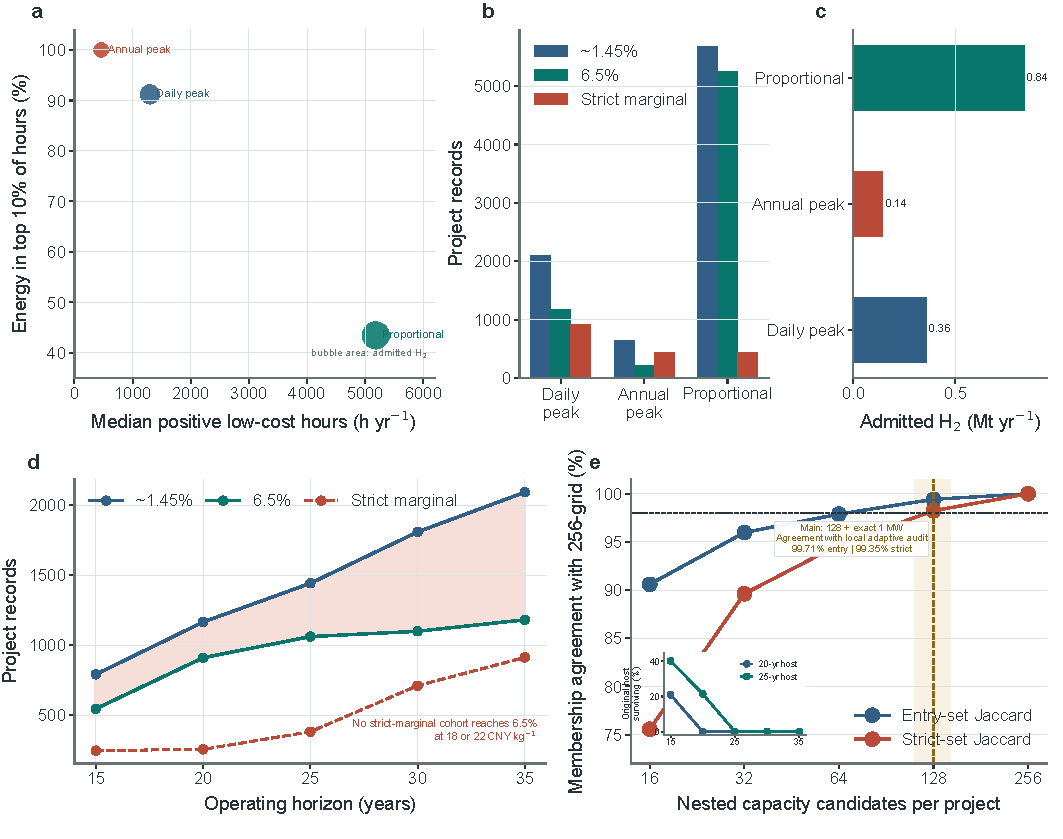
\includegraphics[width=\textwidth]{figures/Supplementary_Figure_S1.pdf}
\caption{Hourly reconstruction, operating horizon and capacity-search choices alter exact entry counts but not the return-separation mechanism. \textbf{a}, Temporal concentration under daily-peak, annual-peak and proportional constrained-electricity proxies; bubble area represents admitted hydrogen. \textbf{b}, Low-return, 6.5\% and strict-marginal record counts for the three proxies. \textbf{c}, Admitted annual hydrogen under each proxy. \textbf{d}, Independently reoptimised entry and strict-marginal counts across 15--35-year operating horizons; no horizon-specific strict-marginal cohort reaches durable 6.5\% at 18 or 22\,CNY\,kg$^{-1}$. \textbf{e}, Membership agreement with the 256-candidate reference as capacity-search density increases; the dashed marker denotes the selected 128-resource-candidate specification before insertion of the exact 1-MW engineering boundary. The inset reports the share of original host records that remain within 20- and 25-year age screens. All counts are deterministic model classifications.}
\label{fig:robustness}
\end{figure}

\begin{figure}[p]
\centering
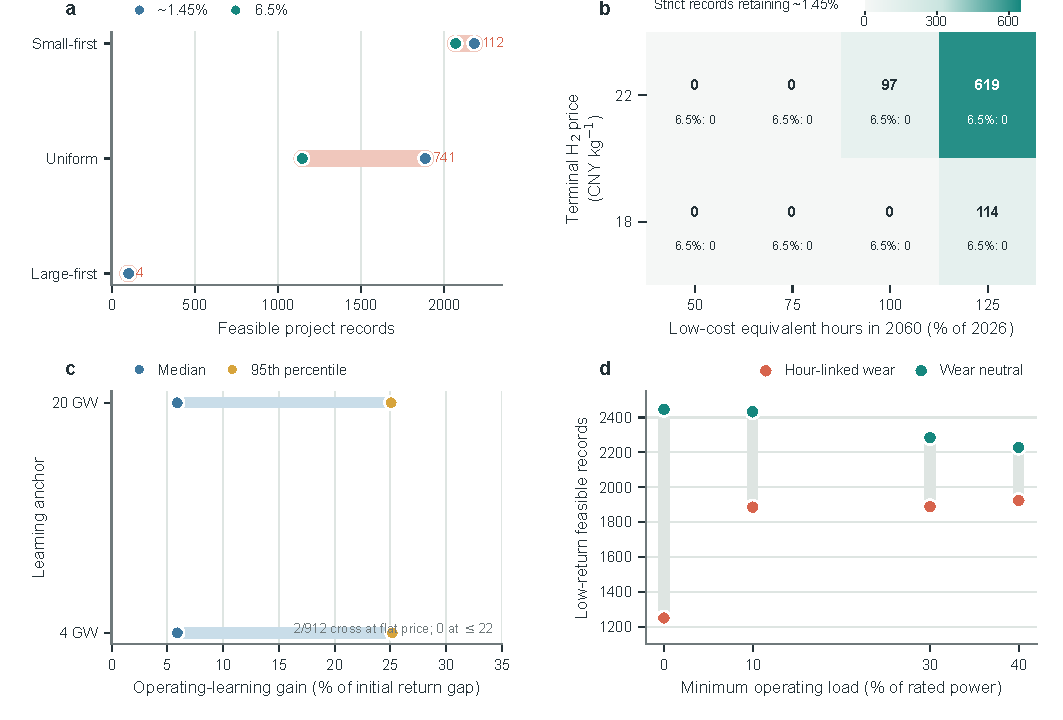
\includegraphics[width=\textwidth]{figures/Supplementary_Figure_S2.pdf}
\caption{High-risk boundary tests separate uncertainty in exact cohort size from robustness of the return-separation mechanism. \textbf{a}, Low-return and 6.5\%-feasible records under province--technology energy-conserving allocation extremes; coral spans are strict-marginal cohorts and labels give their sizes. \textbf{b}, Strict-marginal records retaining the low-return criterion under linear lifetime resource-access paths and terminal producer prices; every cell has zero durable 6.5\% upgrades. \textbf{c}, Median and 95th-percentile incumbent-learning gains relative to initial return gaps when cumulative global electrolysis is anchored at 4 or 20\,GW; the arrow locates the out-of-range 100\% closure boundary. \textbf{d}, Low-return entry across alkaline minimum-load assumptions with standard hour-linked degradation and replacement accounting or a wear-neutral counterfactual. All panels use deterministic stress tests and do not represent probability intervals.}
\label{fig:highrisk}
\end{figure}

\begin{figure}[p]
\centering
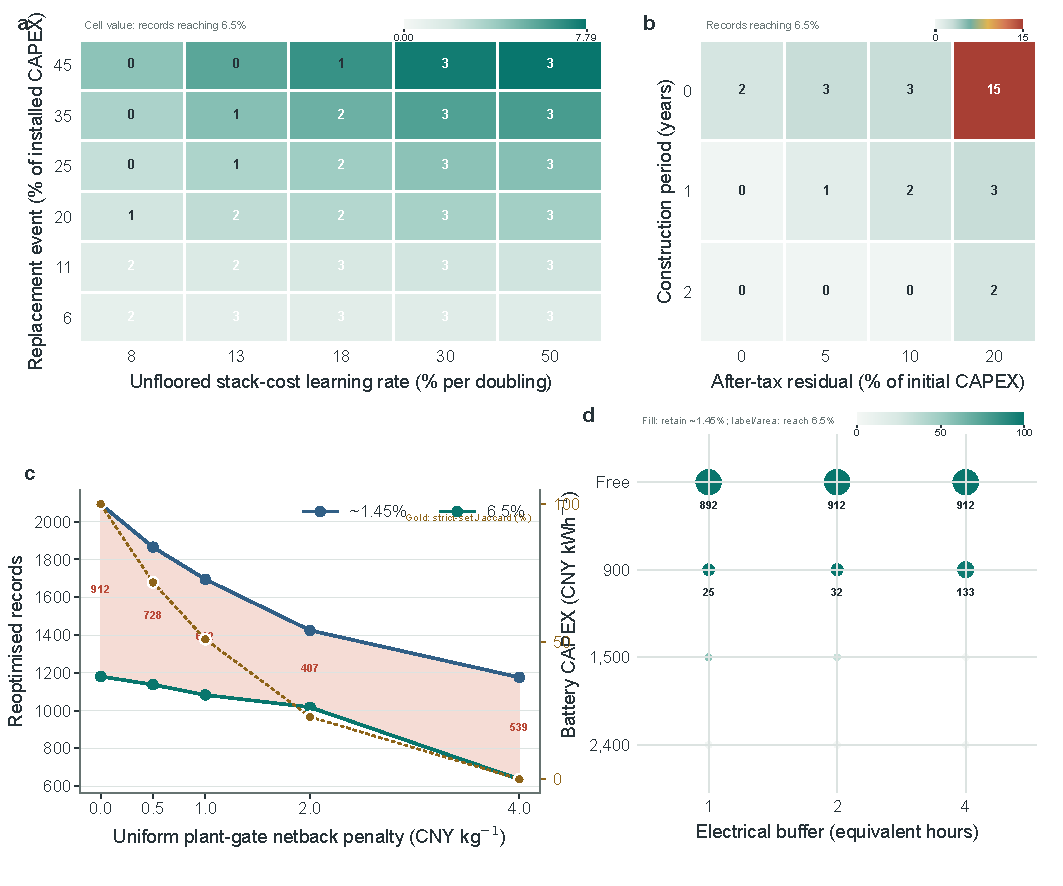
\includegraphics[width=\textwidth]{figures/Supplementary_Figure_S3.pdf}
\caption{Boundary tests distinguish robustness of the vintage-learning mechanism from sensitivity of the selected cohort. \textbf{a}, Strict-marginal records reaching 6.5\% across unfloored stack-cost learning rates and event replacement-cost shares at a fixed 60,000-h cadence. \textbf{b}, Records reaching 6.5\% after adding construction duration and after-tax residual value to the central operating-learning case. \textbf{c}, Reoptimised low-return, 6.5\%-feasible and strict-marginal counts under uniform producer-side netback penalties; the line gives Jaccard agreement of strict membership with the zero-penalty cohort. \textbf{d}, Records retaining the low-return criterion and reaching 6.5\% under free lossless and costed electrical-buffer cases; the central costed specification uses 1,500\,CNY\,kWh$^{-1}$, 85\% round-trip efficiency, 15-year life and full replacement. All tests are deterministic boundaries rather than probability estimates.}
\label{fig:newboundaries}
\end{figure}

\begin{figure}[p]
\centering
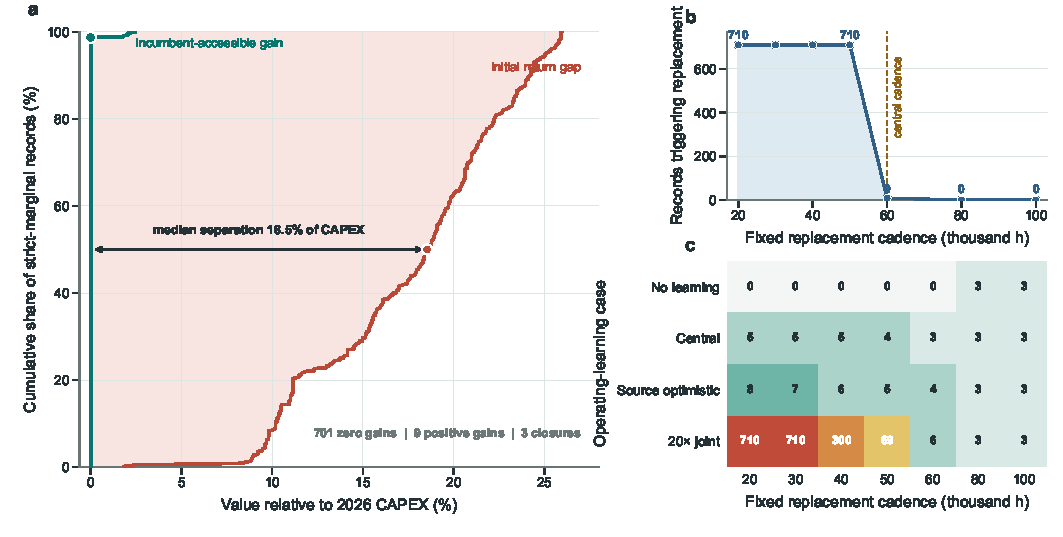
\includegraphics[width=\textwidth]{figures/Supplementary_Figure_S4.pdf}
\caption{Replacement timing separates physical access to operating learning from the sufficiency of its financial payoff. \textbf{a}, Empirical cumulative distributions of the initial 6.5\% NPV gap and central replacement-mediated operating gain across 710 strict-marginal records on the same 2026-CAPEX scale. \textbf{b}, Records triggering at least one replacement over 30 years under fixed replacement cadences; the dashed line marks the central 60,000-hour assumption. \textbf{c}, Records reaching 6.5\% under no learning, central learning, source-informed optimistic learning and a twenty-fold joint-improvement stress. At 80,000--100,000 hours no record replaces; the three classifications above 6.5\% therefore reflect avoided replacement expenditure rather than captured learning. All cases are deterministic counterfactuals.}
\label{fig:replacementgate}
\end{figure}

\clearpage
\addcontentsline{toc}{section}{Supplementary data and reporting checklist}
{\scriptsize
\begin{longtable}{>{\raggedright\arraybackslash}p{0.39\textwidth}>{\raggedright\arraybackslash}p{0.54\textwidth}}
\caption{\textbf{Supplementary data and reporting checklist.} Machine-readable files packaged with this Supplementary Information.}\label{tab:files}\\
\toprule
File & Contents \\
\midrule
\endfirsthead
\multicolumn{2}{l}{\textit{Table \thetable\ continued}}\\
\toprule
File & Contents \\
\midrule
\endhead
\bottomrule
\endfoot
\path{headline_results.json} & M129 headline counts, capacity, capital, hydrogen, learning and R4 outcomes \\
\path{parameter_provenance_registry.csv} & Main values, sensitivity bounds, evidence class, source and required interpretation for each consequential parameter \\
\path{external_source_registry.csv} & Retrieval URLs, analytical roles, file sizes, licence notes and SHA-256 hashes for the external transport, water and IEA project inputs \\
\path{hourly_input_provenance.csv}; \path{hourly_input_hashes.csv} & Laboratory origin, earlier article and code commit, dimensions, identifier matching and SHA-256 hashes for hourly inputs \\
\path{station_inventory_coverage_benchmark.csv}; \path{chinabond_government_5y_20260604_20260702.csv} & Official-capacity coverage calculation and the 20 daily observations underlying the nominal low-return anchor \\
\path{provincial_utilization_2021_2025_harmonized.csv}; \path{monthly_utilization_validation_*} & Harmonised annual panel, 42 monthly comparisons and validation metrics \\
\path{timestamp_timezone_diagnostic.csv}; \path{electrolyser_deployment_authoritative_anchors.csv}; \path{dynamic_parameter_provenance.csv} & Timestamp interpretation check, external deployment benchmarks and a parameter-by-parameter record of citations, construction rules and inferential status \\
\path{provincial_water_price_input.csv} & Complete province and market-region water-price table reused from the earlier Supplementary Table 3 \\
\path{learning_paths_2026_2060.csv} & Annual deployment, cost, efficiency and stack-life trajectories read by the financial model \\
\path{R1_capture_frontier_verified.csv} & Physical capture, capacity and hydrogen-production frontier \\
\path{R2_continuous_hurdle_frontier_dense128.csv}; \path{R2_entry_price_sensitivity_dense128.csv}; \path{R2_R3_return_ladder_learning_M129_30y.csv} & M129 continuous return-criterion frontier, entry-price sensitivity and locked-capacity learning transitions across seven return-gap pairs \\
\path{external_financing_hurdle_ladder_M129.csv}; \path{IEA_China_electrolysis_status_summary.csv} & Exact M129 return counts at five financing contexts and public IEA status counts for located Chinese electrolysis projects \\
\path{M129_station_entry_results.csv}; \path{M129_province_exposure.csv}; \path{M129_hourly_proxy_full_chain_summary.csv}; \path{M129_horizon_full_chain.csv}; \path{M129_host_asset_continuity_screen.csv}; \path{M129_project_record_identity_audit.csv}; \path{M129_capacity_grid_convergence.csv}; \path{M129_engineering_boundary_continuous_summary.json} & Record-level entry, provincial exposure, hourly-allocation, horizon, host-continuity, project-record identity, capacity-grid and continuous-search audits \\
\path{R3_learning_gain_vs_gap_dense128.csv}; \path{R3_operating_hours_replacement_diagnostic_dense128.csv}; \path{R3_learning_flip_boundary_dense128.csv}; \path{R3_learning_intensity_curve_dense128.csv}; \path{R3_critical_terminal_price_dense128.csv}; \path{R3_mechanism_counterfactual_dense128.json}; \path{R3_price_path_summary_dense128.csv}; \path{R3_replacement_cadence_dense128.csv} & M129 operating-hour and replacement-event audit, gap distributions, flip boundary, replacement cadence, critical prices, paired NPV counterfactuals and terminal-price timing outcomes \\
\path{R3_component_incidence_path_M129.csv}; \path{R3_nonstack_transfer_price_passthrough_M129.csv}; \path{R3_incidence_joint_boundary_M129.csv}; \path{R3_critical_nonstack_transfer_share_M129.csv}; \path{R3_incumbent_access_price_passthrough_M129.csv}; \path{R3_price_passthrough_weight_sensitivity_M129.csv}; \path{R3_stack_learning_rate_cadence_surface_M129.csv}; \path{R3_critical_stack_learning_rate_M129.csv}; \path{R3_stack_scope_learning_sensitivity_M129.csv} & Component incidence, joint component-share--learning--price boundary, central non-stack transfer--price-pass-through surface, auxiliary incumbent access, unfloored stack-learning-rate--cadence surface, record-level critical boundaries and replacement-cost-scope sensitivity \\
\path{R4_capacity_flexibility_dense128.csv}; \path{S27_R4_minimum_build_size_sensitivity_M129.csv}; \path{R4_durability_frontier_dense128.csv}; \path{R4_support_requirements_dense128.csv} & M129 pre-investment flexibility, minimum-build discontinuity audit, durability frontier and support requirements \\
\path{G16_R4_actual_weather_capacity_flexibility.csv} & Six-weather-year pre-investment flexibility replay using the separate G16 denominator \\
\path{ERA5_multiyear_headline.json}; \path{R2_entry_summary_by_era5_weather_year.csv}; \path{R3_mechanism_by_era5_weather_year.csv} & Six-weather-year full-chain entry, return-gap, learning-gain and price-loss results \\
\path{G16_R2_deterministic_scenario_grid.csv} & Complete 972-case curtailed and 324-case full-output deterministic grids; G16 denominators only \\
\path{G16_R2_financing_surface.csv}; \path{G16_R2_horizon_inflation.csv}; \path{G16_R2_alkaline_minimum_load.csv}; \path{G16_R2_minimum_build_size.csv}; \path{G16_R2_water_requirement.csv}; \path{G16_R2_project_record_identity_audit.csv}; \path{G16_R2_host_lifetime_screen.csv} & Financing, inflation, operating horizon, minimum load, minimum build size, water, identity and host-lifetime sensitivities; all retain G16 denominators \\
\path{G16_PEM_static_entry.csv}; \path{PEM_M129_static_entry.csv}; \path{PEM_M129_incumbent_learning_upper_bound.csv} & Legacy G16 PEM boundary, full M129 PEM replication and deliberately favourable incumbent-learning bound \\
\path{G16_R3_horizon_overhaul_degradation.csv} & Horizon, mid-life BOP overhaul and degradation sensitivity \\
\path{S20_spatial_allocation_partial_identification.csv}; \path{S20_station_spatial_allocation_rates.csv} & Province--technology energy-conserving allocation extremes and record-level allocated rates \\
\path{S21_learning_start_anchor_sensitivity.csv}; \path{S21_learning_start_anchor_sensitivity_M129.csv}; \path{S21_learning_start_anchor_sources.csv} & G16 and M129 learning-start checks at 4 and 20 GW and their external deployment anchors \\
\path{S22_resource_persistence_paths.csv}; \path{S22_resource_persistence_paths_M129.csv} & G16 and M129 lifetime low-cost-electricity persistence paths \\
\path{S23_minimum_load_mechanism_audit.csv} & Common-grid minimum-load comparison with and without hour-linked wear \\
\path{S24_construction_residual_sensitivity_M129.csv}; \path{S24_transport_netback_sensitivity_M129.csv}; \path{S24_electrical_buffer_sensitivity_M129.csv} & Construction-duration and residual-value boundary, producer-side netback reoptimisation and free/costed electrical-buffer sensitivity \\
\path{spatial_transport_netback_reoptimization_M129.csv}; \path{spatial_demand_overlap_by_province.csv}; \path{spatial_water_exposure_by_province.csv} & China-specific literature-transfer netback, provincial demand overlap and province-weighted water-constraint exposure \\
\path{joint_uncertainty_priors.json}; \path{joint_uncertainty_summary.csv}; \path{joint_uncertainty_convergence.csv}; \path{joint_uncertainty_record_probabilities.csv} & Declared priors, prior-sensitive cohort outcomes, convergence diagnostics and record-level assumption-weighted shares \\
\end{longtable}
}
\FloatBarrier

\begin{table}[!h]
\caption{Statements that should and should not be made from the model.}\label{tab:claims}
\centering
\footnotesize
\begin{tabularx}{\textwidth}{>{\raggedright\arraybackslash}X>{\raggedright\arraybackslash}X}
\toprule
Supported statement & Unsupported extrapolation \\
\midrule
Within the specified GEM inventory, constrained-electricity availability is much smaller than the full-output physical upper bound. & China has exactly 1.29\,Mt\,yr$^{-1}$ of national curtailed-electricity hydrogen potential. \\
Different publicly disclosed enterprise criteria create different modelled entry sets and a measurable but smaller increment of capacity, capital and output. & Approximately 1.45\% is a statutory nationwide approval threshold or a rule followed by all state-owned energy enterprises. \\
Operating learning available to 2026 incumbents closes very few strict-marginal return gaps under the specified bounds. & Technology learning cannot improve any future hydrogen project. \\
Price endpoints and timing condition incumbent durability. & The model forecasts the probability of a particular 2060 hydrogen price. \\
Declared-prior propagation quantifies assumption-weighted durability and its prior sensitivity. & These conditional values are not observed project-success rates or calibrated FID probabilities. \\
Forward screening and pre-investment resizing reduce capital exposure in deterministic scenarios. & The model identifies the socially optimal subsidy or predicts actual programme uptake. \\
Production-side results are an optimistic revenue boundary. & Every modelled kilogram can be sold locally without storage, transport or demand constraints. \\
\bottomrule
\end{tabularx}
\end{table}
\FloatBarrier

\begingroup
\footnotesize
\setlength{\LTleft}{0pt}
\setlength{\LTright}{0pt}
\begin{longtable}{>{\raggedright\arraybackslash}p{0.19\textwidth}>{\raggedright\arraybackslash}p{0.43\textwidth}>{\raggedright\arraybackslash}p{0.28\textwidth}}
\multicolumn{3}{l}{\label{tab:questionaudit}\textbf{Table S12.} Reviewer-facing interpretation audit.}\\[0.4em]
\toprule
Question & Answer supported by the present analysis & Remaining boundary or required evidence \\
\midrule
\endfirsthead
\multicolumn{3}{l}{\emph{Table S12 continued}}\\
\toprule
Question & Answer supported by the present analysis & Remaining boundary or required evidence \\
\midrule
\endhead
\bottomrule
\endfoot
\bottomrule
\endlastfoot
Does the lower firm rule represent a rational equity cost or national policy? & No. It is an observed firm-level institutional scenario. The 1--10\% continuous frontier and seven return-ladder pairs show how conclusions change without assigning normative status to either disclosed rule. Exact M129 revaluation qualifies 1,255 records at the IEA's 2021 4.9\% nominal utility-solar cost-of-capital context for China, 1,099 at 6.5\%, 1,036 at 8\% and 874 at 10\%. & Actual final investment decisions require project-specific green-hydrogen WACC, governance constraints and financing approval data; 4.9\% is contextual rather than a hydrogen WACC. \\
Is failure to reach 6.5\% a mechanical consequence of cohort definition? & No. Central learning upgrades 29 of 40 records in the narrow 6.0--6.5\% band, showing that the model permits reversal. Of the 710 main strict records, 704 remain unresolved at 20 times central combined learning; cohort-wide reversal occurs only when extreme joint learning is paired with 20,000--30,000-h replacement. & The tests identify deterministic thresholds, not empirical frequencies of future learning outcomes. \\
Is exogenous hydrogen-price decline the only reason early assets underperform? & No. At a constant 28\,CNY\,kg$^{-1}$ price, central incumbent learning upgrades three of 710 records and full favourable non-stack transfer upgrades at most eight. Price convergence is separately shown to dominate subsequent NPV loss. & Terminal prices and timing are conditional paths; their probability is not estimated. \\
What does the 28\,CNY\,kg$^{-1}$ value represent? & It is a producer-side reference anchored to a December 2024 cross-route market sample and used as a static rule-isolation counterfactual. Entry-price sensitivity from 18 to 32\,CNY\,kg$^{-1}$ shows its influence on cohort size. & It is not represented as a dedicated green-hydrogen long-term contract or a forecast of one national price. \\
Which provinces lie closest to the modelled 6.5\% boundary? & For provinces with at least ten strict records, median critical 2060 plant-gate prices range from 33.7--35.0\,CNY\,kg$^{-1}$ in Heilongjiang, Shandong and Inner Mongolia to 38.4--41.0 in Qinghai, Xinjiang, Hebei, Shanxi and Hunan. & These rankings exclude route-specific netback, demand and basin-water feasibility and must not be read as delivered-cost rankings. \\
Are physical resource and hourly allocation observed? & Annual province--technology constrained-energy totals are officially calibrated; monthly monitoring and six ERA5 years provide seasonal and meteorological checks. Three hourly proxies and two within-group allocation extremes quantify structural uncertainty. & Unit-level constrained dispatch is not observed, so exact record membership and provincial exposure are only partially identified. \\
Are nominal and real financial quantities internally consistent? & Yes. Constant-2026-CNY revenues and costs are escalated by a common inflation rate before nominal debt service and nominal return criteria are applied. Inflation, debt share, loan rate, horizon, construction and residual-value tests are reported separately. & Debt-service coverage, reserve accounts, covenant breach, default and refinancing are outside the return screen, so qualification is not bankability. \\
Does the inventory support a national potential estimate? & No. It covers approximately 72\% of the contemporaneous all-wind-plus-centralized-photovoltaic benchmark and 53\% of the broader denominator including distributed photovoltaics. All absolute quantities are explicitly inventory-conditioned. & The missing inventory is non-random; national scaling would require a complete asset census or an empirically defensible sampling design. \\
Can all modelled hydrogen be sold locally? & This is not established. The main result is a complete plant-gate-sales upper bound. Transferring province storage-and-transport costs from an independent Chinese supply-chain model reduces lower-rule and 6.5\%-feasible records to 331 and 93 and changes strict membership completely. & The transfer is not a route quotation. Project-specific throughput, storage, contracts, offtake credit and local industrial absorption remain unidentified. \\
Are deterministic scenario shares investment probabilities? & No. All 1,296 broad-grid cases retain equal diagnostic status. A separate 5,000-draw-per-case audit declares priors and dependence explicitly; its reference plant-gate project--draw share is 0.0367\%, with 0.0225--0.0929\% across prior tests. & These are prior-sensitive weighted shares, not empirical probabilities. Empirical FID probabilities require historically calibrated joint distributions and out-of-sample validation. \\
Could storage reverse the direct-coupling result? & A free lossless one-hour buffer upgrades all 710 records, proving that perfect flexibility can reverse the classification. Source-central costed one-, two- and four-hour battery cases upgrade none, separating electrolyser learning from a new storage investment. & Site-specific storage design, hydrogen buffering and market co-optimisation remain outside the primary configuration. \\
Are water constraints represented? & Provincial water prices and 10--60\,kg-water-per-kg-H$_2$ direct-cost sensitivity are included. An external 2,853-county study implies province-weighted 2030 exposure equivalent to 312 strict records, 0.69\,GW and 0.021\,Mt\,yr$^{-1}$. & County identities, basin availability, seasonal scarcity, abstraction permits and competing uses are not matched to records; no station-level exclusion is inferred. \\
Do alkaline results generalise to PEM and full-output electrolysis? & Full M129 PEM reoptimisation gives 3,498/1,826, 700/101 and 2/0 lower-rule/6.5\% counts across favourable, central and adverse bundles. A deliberately favourable PEM incumbent-learning bound upgrades 8 of 636 strict records. Full output remains a separate opportunity-cost branch. & PEM results are technology-specific conditional bounds, not a cross-country validation or evidence that all PEM projects share one parameter bundle. \\
Does pre-investment flexibility rescue sunk assets? & No. Capacity flexibility creates value only before commitment. Without a minimum-build cutoff, 25\% adjustability at 75\% resource realisation reduces exposed capital from 1.18 to 0.61\,billion CNY. At 50\%, exposure is removed while 91.3\% of locked output is retained and output from records reaching 6.5\% increases from 0.105 to 0.169\,Mt\,yr$^{-1}$. The zero exposure reported at 25\% under the 1-MW convention results from mapping 154 sub-threshold capacities to no-build. & Minimum viable scale, cancellation costs, permitting, interconnection queues, modular procurement and information arrival are required for an implementable real-option valuation. \\
Does the model identify an optimal subsidy? & No. Price-premium and capital-grant calculations report the financing gap after capacity is locked; their magnitudes show why broad retrospective rescue is expensive. & Welfare, fiscal incidence, downstream decarbonisation value, information rents and programme uptake are required for optimal policy design. \\
\end{longtable}
\endgroup
\FloatBarrier

\section*{Data availability}

Publicly redistributable project metadata, annual utilisation inputs, processed ERA5 outputs, parameter provenance, figure source data and result tables are maintained in the accompanying GitHub repository at \href{https://github.com/1223044298-ship-it/curtailment-traps-early-green-hydrogen-assets-beyond-the-reach-of-learning}{github.com/1223044298-ship-it/curtailment-traps-early-green-hydrogen-assets-beyond-the-reach-of-learning}. The repository is private during manuscript review. The manuscript-aligned revision is identified by a fixed Git commit, and repository access will be supplied to editors and reviewers; the accepted release will be made public and archived under a versioned DOI before publication. Source ERA5 variables are publicly available from the Copernicus Climate Data Store under its applicable terms. The 2020 monthly model-output files were generated within the authors' research group, previously used and documented by Li and Zhang\cite{li2026}, and reused here. Their lineage is fixed to that article and its public source-code repository at commit \texttt{43af9fe}. The source-study code reads, but does not distribute or regenerate, those files. The two 10,214-by-8,784 hourly profile arrays used here are deterministic derivatives of the monthly inputs. The monthly files and derived arrays required for a clean raw-to-results rerun are not redistributed in the repository. They are held by the authors' research group and documented by filename, analytical role, dimension, SHA-256 checksum, identifier matching and transformation code. Requests for research access should be sent to the corresponding author at \href{mailto:h.zhang@pku.edu.cn}{h.zhang@pku.edu.cn} and should identify the intended research use; access is subject to contributor and institutional approval and applicable data-sharing conditions. Inputs subject to source licences are documented by provider, release date, licence and retrieval route. The packaged derived outputs support reproduction of all figures and numerical auditing of the reported results but do not, without the request-access inputs, constitute a complete raw-to-results archive.

\section*{Code availability}

Custom code for hourly constrained-electricity reconstruction, ERA5 replay, capacity optimisation, nominal equity cash flow, learning-flip boundaries, forward screening, capacity flexibility and figure generation is maintained in the accompanying GitHub repository. The submission snapshot includes environment specifications, execution order, an input inventory and SHA-256 manifests. The request-access inputs needed for a clean raw-to-results rerun are listed explicitly in \texttt{analysis\_code/INPUTS\_REQUIRED.csv}. No archival DOI has yet been assigned; the accepted public release will receive a versioned archival DOI before publication.

\section*{Supplementary references}

\begin{thebibliography}{99}

\bibitem{gem2024}
Global Energy Monitor. \emph{Global Wind Power Tracker} and \emph{Global Solar Power Tracker}, June 2024 releases (2024). \href{https://globalenergymonitor.org/projects/global-wind-power-tracker/}{Wind tracker}; \href{https://globalenergymonitor.org/projects/global-solar-power-tracker/}{solar tracker}.

\bibitem{nea2024capacity}
National Energy Administration. \emph{National Electric Power Industry Statistics and Photovoltaic Construction, January--June 2024} (20 and 25 July 2024, in Chinese). \href{https://www.nea.gov.cn/2024-07/20/c_1310782235.htm}{Power statistics}; \href{https://www.nea.gov.cn/2024-07/25/c_1310782757.htm}{photovoltaic breakdown}.

\bibitem{osmcoast}
OpenStreetMap contributors. \emph{OpenStreetMap administrative relations and coastline-derived land polygons} (data timestamp 28 August 2026). \href{https://www.openstreetmap.org/copyright}{Copyright and ODbL licence}; \href{https://osmdata.openstreetmap.de/data/land-polygons.html}{land polygons}.

\bibitem{mnrmap2023}
Ministry of Natural Resources of the People's Republic of China. \emph{China boundary map, 1:7,400,000, standard-map product GS(2023)2767} (Standard Map Service System, 2023). \href{http://bzdt.ch.mnr.gov.cn/}{Official portal}.

\bibitem{li2026}
Li, Y. \& Zhang, H. Can renewable hydrogen blending support a nationwide pathway in China? \emph{Nexus} \textbf{3}, 100149 (2026). \href{https://doi.org/10.1016/j.ynexs.2026.100149}{doi: 10.1016/j.ynexs.2026.100149}.

\bibitem{renewable2025}
Electric Power Planning, Research, Monitoring and Early-Warning Center. \emph{National New Energy Grid Integration and Consumption, 2025} (table republished by China Energy News, 9 February 2026, in Chinese). \href{https://epaper.ceic.com/pad/content/202602/09/content_20205.html}{Annual provincial table}; \href{https://www.xnyxnyj.cn/}{monitoring portal}.

\bibitem{hersbach2020}
Hersbach, H. \emph{et al.} The ERA5 global reanalysis. \emph{Q. J. R. Meteorol. Soc.} \textbf{146}, 1999--2049 (2020). \href{https://doi.org/10.1002/qj.3803}{doi: 10.1002/qj.3803}.

\bibitem{era5data}
Copernicus Climate Change Service. \emph{ERA5 hourly data on single levels from 1940 to present} (accessed 12 August 2026). \href{https://doi.org/10.24381/cds.adbb2d47}{doi: 10.24381/cds.adbb2d47}.

\bibitem{worldbank2026}
Energy Sector Management Assistance Program. \emph{Electrolyzers for Hydrogen Production: Technical and Economic Characteristics}, ESMAP Technical Report No. 208469 (World Bank, Washington, DC, 2026). \href{https://doi.org/10.1596/44443}{doi: 10.1596/44443}.

\bibitem{iea2025}
International Energy Agency. \emph{Global Hydrogen Review 2025} (IEA, Paris, 2025). \href{https://www.iea.org/reports/global-hydrogen-review-2025}{Official report}.

\bibitem{doe2024}
Hubert, M., Esposito, A. M., Peterson, D., Miller, E. \& Stanford, J. \emph{Hydrogen Shot: Water Electrolysis Technology Assessment} (US Department of Energy, Hydrogen and Fuel Cell Technologies Office, 2024). \href{https://www.energy.gov/sites/default/files/2024-12/hydrogen-shot-water-electrolysis-technology-assessment.pdf}{Official report}.

\bibitem{changyuan2026}
CHN Energy Changyuan Electric Power Co., Ltd. \emph{Investment Management Measures, 3rd edn}, Annex 1 (26 June 2026, in Chinese). \href{https://static.cninfo.com.cn/finalpage/2026-06-26/1225388602.PDF}{Official disclosure}.

\bibitem{huadian2025}
Huadian Energy Co., Ltd. \emph{Investment Management Regulations}, Annex 1 (6 December 2025, in Chinese). \href{https://static.cninfo.com.cn/finalpage/2025-12-06/1224855581.PDF}{Official disclosure}.

\bibitem{chinabond2026}
China Central Depository \& Clearing Co., Ltd. \emph{ChinaBond five-year government bond yield curve}, 4 June--2 July 2026 (2026). \href{https://yield.chinabond.com.cn/cbweb-pbc-web/pbc/historyQuery?startDate=2026-06-04\&endDate=2026-07-02\&gjqx=0\&qxId=ycqx}{Exact 20-trading-day query}.

\bibitem{nea2025hydrogen}
National Energy Administration \& CHN Energy Hydrogen Innovation Technology Co., Ltd. \emph{China Hydrogen Development Report 2025} (30 April 2025, in Chinese). \href{https://www.nea.gov.cn/20250430/96022785b3a747248288ad1c57d3a025/c.html}{Official report}.

\bibitem{renewableannual}
National Energy Administration. \emph{Renewable Energy Power Development and Utilisation Monitoring Results, 2021--2024} (2022--2025, in Chinese). \href{https://www.nea.gov.cn/2022-09/16/c_1310663387.htm}{2021}; \href{https://zfxxgk.nea.gov.cn/2023-09/07/c_1310741874.htm}{2022}; \href{https://zfxxgk.nea.gov.cn/2024-10/10/c_1310787115.htm}{2023}; \href{https://www.nea.gov.cn/20251113/cc1fb0298a2944f8bd5441f67c9be9b3/c.html}{2024}.

\bibitem{renewablemonthly}
National New Energy Consumption Monitoring and Early Warning Center. \emph{National New Energy Grid Integration and Consumption: August, September and November 2025} (tables republished by China Energy News, 2025--2026, in Chinese). \href{https://epaper.ceic.com/pc/attachment/202510/13/26e6af76-e1b7-40fb-b126-bc59f391e51c.pdf}{August table}; \href{https://epaper.ceic.com/pc/attachment/202511/07/6063762d-43ea-41fc-a37d-5f5549f62a5d.pdf}{September table}; \href{https://epaper.ceic.com/pc/attachment/202601/12/bf2a9f58-b724-435d-8c46-447e3ebbdc3d.pdf}{November table}.

\bibitem{irena2020}
International Renewable Energy Agency. \emph{Green Hydrogen Cost Reduction: Scaling up Electrolysers to Meet the 1.5\,$^\circ$C Climate Goal} (IRENA, Abu Dhabi, 2020). \href{https://www.irena.org/-/media/Files/IRENA/Agency/Publication/2020/Dec/IRENA_Green_hydrogen_cost_2020.pdf}{Official report}.

\bibitem{gov2026}
State Council of the People's Republic of China. \emph{Report on the Work of the Government} (5 March 2026, in Chinese). \href{https://www.npc.gov.cn/c2/c30834/202603/t20260316_453264.html}{Official report}.

\bibitem{taxlaw}
National People's Congress \& State Council of the People's Republic of China. \emph{Enterprise Income Tax Law of the People's Republic of China and Implementing Regulations} (current versions, in Chinese). \href{https://flk.npc.gov.cn/detail?id=ff8080816f135f46016f2106acd11784}{Law}; \href{https://policy.mofcom.gov.cn/claw/clawContent.shtml?id=102338}{implementing regulations}.

\bibitem{iea2026}
International Energy Agency. \emph{Global Hydrogen Review 2026} (IEA, Paris, 2026). \href{https://www.iea.org/reports/global-hydrogen-review-2026}{Official report}.

\bibitem{ieaelectrolysers2024}
International Energy Agency. \emph{Electrolysers} (IEA, Paris, 2024). \href{https://www.iea.org/energy-system/hydrogen/electrolysers}{Official analysis and project-pipeline data}.

\bibitem{iea2023nze}
International Energy Agency. \emph{Hydrogen: Tracking Clean Energy Progress} (IEA, Paris, 2023). \href{https://www.iea.org/reports/hydrogen-2156}{Official Net Zero Emissions pathway milestones}.

\bibitem{iea2021minerals}
International Energy Agency. \emph{The Role of Critical Minerals in Clean Energy Transitions} (IEA, Paris, 2021). \href{https://www.iea.org/reports/the-role-of-critical-minerals-in-clean-energy-transitions/mineral-requirements-for-clean-energy-transitions}{Official Sustainable Development Scenario analysis}.

\bibitem{irena2023}
International Renewable Energy Agency. \emph{World Energy Transitions Outlook 2023: 1.5$^{\circ}$C Pathway} (IRENA, Abu Dhabi, 2023). \href{https://www.irena.org/Publications/2023/Jun/World-Energy-Transitions-Outlook-2023}{Official report}.

\bibitem{odenweller2025}
Odenweller, A. \& Ueckerdt, F. The green hydrogen ambition and implementation gap. \emph{Nat. Energy} \textbf{10}, 110--123 (2025). \href{https://doi.org/10.1038/s41560-024-01684-7}{doi: 10.1038/s41560-024-01684-7}.

\bibitem{glenk2023}
Glenk, G., Holler, P. \& Reichelstein, S. Advances in power-to-gas technologies: cost and conversion efficiency. \emph{Energy Environ. Sci.} \textbf{16}, 6058--6070 (2023). \href{https://doi.org/10.1039/D3EE01208E}{doi: 10.1039/D3EE01208E}.

\bibitem{ferioli2009}
Ferioli, F., Schoots, K. \& van der Zwaan, B. C. C. Use and limitations of learning curves for energy technology policy: a component-learning hypothesis. \emph{Energy Policy} \textbf{37}, 2525--2535 (2009). \href{https://doi.org/10.1016/j.enpol.2008.10.043}{doi: 10.1016/j.enpol.2008.10.043}.

\bibitem{zeyen2023}
Zeyen, E., Victoria, M. \& Brown, T. Endogenous learning for green hydrogen in a sector-coupled energy model for Europe. \emph{Nat. Commun.} \textbf{14}, 3743 (2023). \href{https://doi.org/10.1038/s41467-023-39397-2}{doi: 10.1038/s41467-023-39397-2}.

\bibitem{odenweller2022}
Odenweller, A., Ueckerdt, F., Nemet, G. F., Jensterle, M. \& Luderer, G. Probabilistic feasibility space of scaling up green hydrogen supply. \emph{Nat. Energy} \textbf{7}, 854--865 (2022). \href{https://doi.org/10.1038/s41560-022-01097-4}{doi: 10.1038/s41560-022-01097-4}.

\bibitem{irenatransport2022}
International Renewable Energy Agency. \emph{Global Hydrogen Trade to Meet the 1.5\,$^\circ$C Climate Goal: Part II---Technology Review of Hydrogen Carriers} (IRENA, Abu Dhabi, 2022). \href{https://www.irena.org/publications/2022/Apr/Global-hydrogen-trade-Part-II}{Official report}.

\bibitem{bi2026}
Bi, C., Guo, F. \& Zhang, N. Hydrogen supply chains across Chinese provinces for production and transportation. \emph{Commun. Earth Environ.} (2026). \href{https://doi.org/10.1038/s43247-026-03869-2}{doi: 10.1038/s43247-026-03869-2}.

\bibitem{xie2026}
Xie, X. \emph{et al.} Addressing water resource constraints for electrolytic hydrogen demand in China. \emph{Nat. Sustain.} (2026). \href{https://doi.org/10.1038/s41893-026-01894-9}{doi: 10.1038/s41893-026-01894-9}.

\bibitem{cole2023battery}
Cole, W. \& Karmakar, A. \emph{Cost Projections for Utility-Scale Battery Storage: 2023 Update}, NREL/TP-6A40-85332 (National Renewable Energy Laboratory, Golden, 2023). \href{https://www.nrel.gov/docs/fy23osti/85332.pdf}{Official report}.

\bibitem{nrelatb2023}
National Renewable Energy Laboratory. \emph{2023 Annual Technology Baseline: Utility-Scale Battery Storage} (2023). \href{https://atb.nrel.gov/Electricity/2023/2023/utility-scale_battery_storage}{Official data and methods}.

\bibitem{ieaprojects2026}
International Energy Agency. \emph{Hydrogen Production and Infrastructure Projects Database} (IEA, Paris, June 2026 release; accessed 25 August 2026). \href{https://www.iea.org/data-and-statistics/data-product/hydrogen-production-and-infrastructure-projects-database}{Official database}.

\bibitem{ieacapital}
International Energy Agency. \emph{Cost of Capital Observatory: Tools and Analysis} (IEA, Paris; accessed 25 August 2026). \href{https://www.iea.org/reports/cost-of-capital-observatory/tools-and-analysis}{Official data and methods}.

\end{thebibliography}

\end{document}
